% !Mode:: "TeX:UTF-8"

\def\xuewei{Master} % 定义学位 Doctor or Master

\documentclass[cs4size,openany,UTF8]{ctexbook}
\usepackage[a4paper,text={160true mm,234true mm},top=30.5true mm,left=25true mm,head=5true mm,headsep=2.5true mm,foot=8.5true mm]{geometry}
\usepackage{booktabs}
\usepackage{longtable}
\usepackage{caption}
\usepackage{amsmath}
\usepackage{txfonts}
\usepackage{bm}
\usepackage{graphicx}
\usepackage{enumitem}
\usepackage{fancyhdr}
\usepackage{ntheorem}
\usepackage{titlesec}
\usepackage{subfigure}
\usepackage{tabularx}
\usepackage[sort&compress,numbers]{natbib}
\usepackage[boxed,linesnumbered,algochapter]{algorithm2e}	
\usepackage[unicode,dvipdfmx]{hyperref}
\usepackage{multirow}
\usepackage{rotfloat}

\begin{document}

\newif\ifxueweidoctor
\newif\ifxueweimaster
\def\temp{Doctor}
\ifx\temp\xuewei
  \xueweidoctortrue  \xueweimasterfalse
\fi
\def\temp{Master}
\ifx\temp\xuewei
  \xueweidoctorfalse  \xueweimastertrue
\fi

% !Mode:: "TeX:UTF-8" 
\setlength{\subfigbottomskip}{0pt}
\CTEXoptions[bibname={主要参考文献}]
\CTEXsetup[name={,},number={}]{chapter}
\captionsetup{labelsep=space,font=small,justification=centering}
\arraycolsep=1.7pt
\graphicspath{{figures/}}
\renewcommand{\subcapsize}{\zihao{5}}
\renewcommand{\thesubfigure}{\alph{subfigure})}
\setcounter{secnumdepth}{4}
\newcommand{\pozhehao}{\raisebox{0.1em}{------}}
\titleformat{\chapter}{\center\zihao{-2}\heiti}{\chaptertitlename}{0.5em}{}
\titlespacing{\chapter}{0pt}{-4.5mm}{8mm}
\titleformat{\section}{\zihao{-3}\heiti}{\thesection}{0.5em}{}
\titlespacing{\section}{0pt}{4.5mm}{4.5mm}
\titleformat{\subsection}{\zihao{4}\heiti}{\thesubsection}{0.5em}{}
\titlespacing{\subsection}{0pt}{4mm}{4mm}
\titleformat{\subsubsection}{\zihao{-4}\heiti}{\thesubsubsection}{0.5em}{}
\titlespacing{\subsubsection}{0pt}{0pt}{0pt}
\makeatletter
\renewcommand\thesection{\@arabic \c@section} % 前面不带 thechapter
\makeatother

\theoremstyle{plain}
\theorembodyfont{\songti\rmfamily}
\theoremheaderfont{\heiti\rmfamily}
\newtheorem{definition}{\heiti 定义}
\newtheorem{example}{\heiti 例}
\newtheorem{algo}{\heiti 算法}
\newtheorem{theorem}{\heiti 定理}
\newtheorem{axiom}{\heiti 公理}
\newtheorem{proposition}{\heiti 命题}
\newtheorem{lemma}{\heiti 引理}
\newtheorem{corollary}{\heiti 推论}
\newtheorem{remark}{\heiti 注解}
\newenvironment{proof}{\noindent{\heiti 证明:}}{\hfill $ \square $ \vskip 4mm}
\theoremsymbol{$\square$}

% 定义页眉和页脚 使用fancyhdr 宏包
\newcommand{\makeheadrule}{
\rule[7pt]{\textwidth}{0.75pt} \\[-23pt]
\rule{\textwidth}{2.25pt}}
\renewcommand{\headrule}{
    {\if@fancyplain\let\headrulewidth\plainheadrulewidth\fi
     \makeheadrule}}
\makeatother
		
\pagestyle{fancyplain}
\renewcommand{\chaptermark}[1]{\relax}
\renewcommand{\sectionmark}[1]{\markright{#1}}
\fancyhf{}
\ifxueweidoctor
  \fancyhead[CO]{\songti \zihao{-5}\rightmark}
  \fancyhead[CE]{\songti \zihao{-5} 哈尔滨工业大学博士学位论文开题报告}%
  \fancyfoot[C]{\zihao{-5} -~\thepage~-}
	\renewcommand\bibsection{\section*{\centerline{\bibname}}
	\markboth{哈尔滨工业大学博士学位论文开题报告}{\bibname}}
\fi
\ifxueweimaster
  \fancyhead[C]{\songti \zihao{-5} 哈尔滨工业大学硕士学位论文开题报告}
  \fancyfoot[C]{\zihao{-5} -~\thepage~-}
	\renewcommand\bibsection{\section*{\centerline{\bibname}}
	\markboth{哈尔滨工业大学硕士学位论文开题报告}{\bibname}}
\fi

\renewcommand{\CJKglue}{\hskip 0.56pt plus 0.08\baselineskip} %加大字间距,使每行33个字
\def\defaultfont{\renewcommand{\baselinestretch}{1.62}\normalsize\selectfont}
% 调整罗列环境的布局
\setitemize{leftmargin=3em,itemsep=0em,partopsep=0em,parsep=0em,topsep=-0em}
\setenumerate{leftmargin=3em,itemsep=0em,partopsep=0em,parsep=0em,topsep=0em}
\renewcommand{\theequation}{\arabic{equation}}
\renewcommand{\thetable}{\arabic{table}}
\renewcommand{\thefigure}{\arabic{figure}}

\makeatletter
\renewcommand{\p@subfigure}{\thefigure~}
\makeatother

\newcommand{\citeup}[1]{\textsuperscript{\cite{#1}}} % for WinEdt users

% 封面、摘要、版权、致谢格式定义
\makeatletter
\def\title#1{\def\@title{#1}}\def\@title{}
\def\titlesec#1{\def\@titlesec{& \rule[-4pt]{200pt}{1pt}\hspace{-326pt}\centerline{\textbf{#1}}}}\def\@titlesec{}
\def\affil#1{\def\@affil{#1}}\def\@affil{}
\def\subject#1{\def\@subject{#1}}\def\@subject{}
\def\author#1{\def\@author{#1}}\def\@author{}
\def\bdate#1{\def\@bdate{#1}}\def\@bdate{}
\def\supervisor#1{\def\@supervisor{#1}}\def\@supervisor{}
\def\assosupervisor#1{\def\@assosupervisor{\textbf{副\hfill 导\hfill 师} & \rule[-4pt]{200pt}{1pt}\hspace{-326pt}\centerline{\textbf {#1}}\\}}\def\@assosupervisor{}
\def\cosupervisor#1{\def\@cosupervisor{\textbf{联\hfill 合\hfill 导\hfill 师} & \rule[-4pt]{200pt}{1pt}\hspace{-326pt}\centerline{\textbf {#1}}\\}}\def\@cosupervisor{}
\def\date#1{\def\@date{#1}}\def\@date{}
\def\stuno#1{\def\@stuno{#1}}\def\@stuno{}
% 定义封面
\ifxueweidoctor
\def\makecover{
    \thispagestyle{empty}
    \zihao{-2}\vspace*{10mm}
		\renewcommand{\CJKglue}{\hskip 2pt plus 0.08\baselineskip}
    \centerline{\kaishu\textbf{哈尔滨工业大学}}
		\vspace{10mm}
		\centerline{\zihao{2}\songti\textbf{博士学位论文开题报告}}
		\renewcommand{\CJKglue}{\hskip 0pt plus 0.08\baselineskip}

    \zihao{3}\vspace{2\baselineskip}
    \hspace*{36pt}{\songti
	\renewcommand{\arraystretch}{1.3}
    \begin{tabular}{l@{}l}
    \textbf{院\hfill (系)}   & \rule[-4pt]{200pt}{1pt}\hspace{-326pt}\centerline{\textbf\@affil}\\
    \textbf{学\hfill 科}     & \rule[-4pt]{200pt}{1pt}\hspace{-326pt}\centerline{\textbf\@subject}\\
    \textbf{导\hfill 师}     & \rule[-4pt]{200pt}{1pt}\hspace{-326pt}\centerline{\textbf\@supervisor}\\
    \@assosupervisor
	\@cosupervisor
    \textbf{研\hfill 究\hfill 生}      & \rule[-4pt]{200pt}{1pt}\hspace{-326pt}\centerline{\textbf\@author}\\
    \textbf{入\hfill 学\hfill 时\hfill 间}  & \rule[-4pt]{200pt}{1pt}\hspace{-326pt}\centerline{\textbf\@bdate}\\
    \textbf{开题报告日期} & \rule[-4pt]{200pt}{1pt}\hspace{-326pt}\centerline{\textbf\@date}\\
    \textbf{论\hfill 文\hfill 题\hfill 目}  & \rule[-4pt]{200pt}{1pt}\hspace{-326pt}\centerline{\textbf\@title}\\
    \@titlesec
    \end{tabular}\renewcommand{\arraystretch}{1}}
	\vfill
    \centerline{\songti\textbf{研究生院培养处}}

%%定义内封
\newpage
\thispagestyle{empty}
\zihao{5}\vspace*{2em}
\begin{center}
  \heiti\zihao{3}说\hspace{3em}明
\end{center}
\vspace*{40pt}
	\renewcommand{\arraystretch}{1.25}
    {\songti\zihao{5}
    \hangindent=2em\noindent 一、开题报告应包括下列主要内容:
    \begin{enumerate}[leftmargin=36pt]
    \item 课题来源及研究的目的和意义;
    \item 国内外在该方向的研究现状及分析(文献综述);
    \item 前期的理论研究与试验论证工作的结果;
    \item 学位论文的主要研究内容、实施方案及其可行性论证;
    \item 论文进度安排,预期达到的目标;
    \item 为完成课题已具备和所需的条件、外协计划及经费;
    \item 预计研究过程中可能遇到的困难、问题,以及解决的途径;
    \item 主要参考文献(应在~50~篇以上,其中外文资料不少于二分之一,参考文献中近五年内发表的文献一般不少于三分之一,且必须有近二年内发表的文献资料)。
    \end{enumerate}
    \noindent 二、开题报告字数应不少于~1.5~万字。

    \noindent 三、开题报告时间应最迟应于第四学期结束前完成。

    \hangindent=2em\noindent 四、若本次开题报告未通过,需在三个月内再次进行开题报告。第二次学位论文开题报告
    仍未通过者,将取消其学籍。

    \hangindent=2em\noindent 五、开题报告结束后,评议小组要填写《博士学位论文开题报告评议结果》上报院(系)研
    究生教学秘书备案。

    \noindent 六、此表不够填写时,可另加附页。
    }
	\renewcommand{\arraystretch}{1}
    \clearpage
}
\fi

\ifxueweimaster
\def\makecover{
    \thispagestyle{empty}
    \zihao{-2}\vspace*{10mm}
		\renewcommand{\CJKglue}{\hskip 2pt plus 0.08\baselineskip}
    \centerline{\kaishu\textbf{哈尔滨工业大学}}
		
		\vspace{10mm}
		\centerline{\zihao{2}\songti\textbf{硕士学位论文开题报告}}

		\renewcommand{\CJKglue}{\hskip 0pt plus 0.08\baselineskip}
\vspace{30pt}
\zihao{-2}
\begin{center}\songti\textbf{题~目:\@title}\end{center}
\vspace{30pt}
    \zihao{3}
    \hspace*{68pt}{\songti
	\renewcommand{\arraystretch}{1.3}
    \begin{tabular}{l@{}l}
    \textbf{院\hfill (系)}   & \rule[-4pt]{200pt}{1pt}\hspace{-326pt}\centerline{\textbf\@affil}\\
    \textbf{学\hfill 科}     & \rule[-4pt]{200pt}{1pt}\hspace{-326pt}\centerline{\textbf\@subject}\\
    \textbf{导\hfill 师}     & \rule[-4pt]{200pt}{1pt}\hspace{-326pt}\centerline{\textbf\@supervisor}\\
    \@assosupervisor
	\@cosupervisor
    \textbf{研\hfill 究\hfill 生}      & \rule[-4pt]{200pt}{1pt}\hspace{-326pt}\centerline{\textbf\@author}\\
    \textbf{学\hfill 号}  & \rule[-4pt]{200pt}{1pt}\hspace{-326pt}\centerline{\textbf\@stuno}\\
    \textbf{开题报告日期} & \rule[-4pt]{200pt}{1pt}\hspace{-326pt}\centerline{\textbf\@date}\\
    \end{tabular}
		\renewcommand{\arraystretch}{1}}
	\vfill
    \centerline{\songti\textbf{研究生院培养处制}}
%    \centerline{\songti\textbf{二〇一二年三月}}

%%定义内封
%\newpage
%\thispagestyle{empty}
%\zihao{5}\vspace*{2em}
%\begin{center}
%  \heiti\zihao{3}说\hspace{3em}明
%\end{center}
%\vspace*{40pt}
%	\renewcommand{\arraystretch}{1.25}
%    {\songti\zihao{5}
%    \hangindent=2em
%	\noindent 一、开题报告应包括下列主要内容:
%    \begin{enumerate}[leftmargin=36pt]
%	\item 课题来源及研究的目的和意义;
%	\item 国内外在该方向的研究现状及分析;
%	\item 主要研究内容;
%	\item 研究方案及进度安排,预期达到的目标;
%	\item 为完成课题已具备和所需的条件和经费;
%	\item 预计研究过程中可能遇到的困难和问题,以及解决的措施;
%	\item 主要参考文献。
%    \end{enumerate}
%    \noindent 二、对开题报告的要求
%	\begin{enumerate}[leftmargin=36pt]
%	\item 开题报告的字数应在~5000~字以上;
%	\item 阅读的主要参考文献应在~20~篇以上,其中外文资料应不少于三分之一。硕士研究生应在导师的指导下着重查阅近年内发表的中、\hspace{-1pt}外文期刊文章。\hspace{-1pt}本学科的基础和专业课教材一般不应列为参考资料。
%    \end{enumerate}
%    \noindent 三、开题报告时间应最迟不得超过第三学期的第三周末。
%
%    \hangindent=2em\noindent 四、如硕士生首次开题报告未通过,\hspace{-2pt}需在一个月内再进行一次。\hspace{-3pt}若仍不通过,\hspace{-2pt}则停止硕士论文工作。
%
%    \noindent 五、此表不够填写时,可另加附页。
%
%\hangindent=2em\noindent 六、开题报告进行后,此表同硕士学位论文开题报告评议结果存各系(院)研究生秘书书处,以备研究生院及所属学院进行检查。
%
%    }
%	\renewcommand{\arraystretch}{1}
%    \clearpage
}
\fi
\makeatother
% !Mode:: "TeX:UTF-8" 

\affil{计算机科学与技术}
\subject{计算机科学与技术}
\author{郑伟}
\supervisor{徐晓飞教授}
%\assosupervisor{副导名}%若无副导师,请屏蔽掉此句
%\cosupervisor{联导名}%若无联合导师,请屏蔽掉此句
\date{2012年9月11日}
\stuno{11S003075}
\bdate{2012年9月}

\ifxueweidoctor
  \title{面向不确定性的服务运行时} %论文题目,此处最多12个字,题目剩余的字放在\ctitlesec里面
  \titlesec{决策优化方法}
\fi
\ifxueweimaster
  \title{面向不确定性的服务运行时决策优化方法}
\fi

\makecover
\clearpage
\setcounter{page}{1}
\zihao{-4}

\chapter{基于价值的服务不确定性决策优化}
% !Mode:: "TeX:UTF-8"
\section{课题来源及研究的背景和意义}
\subsection{课题的来源}

服务被定义为客户、提供者、使能者多方之间协同生产~(co-production)~共创价值的过程。例如,软件化服务(如~Web Service)~ 是软件客户端与服务端通过标准化协议(如~SOAP~协议)的交互,客户端发出请求,服务端执行计算任务并将结果返回给客户端;业务服务是现实中的客户方企业与各服务提供企业之间的交互,这种交互既可以是~Internet~支持的网络交互,也可以是现实中的交互。

这意味着,在业务层面上,服务中的任何一方都无法完全控制全局,服务的执行是一个分布式协作的过程。由于无法全局控制,服务的执行不可避免的要面临各种不确定性,不受某一方控制的服务环节可能无法按照其预设的期望来执行。同样,在软件层面上,由于互联网环境的动态变化和不稳定特性,构建在其基础上的服务系统在执行过程中也面临各种不确定性,某些服务环节可能无法按照预期执行,供需双方期望的价值无法完全实现,还可能触发其他更多的不确定性事件,造成各种直接和潜在的影响。

\subsection{课题研究的背景和意义}
本课题将不确定性定义为“某个已经或即将发生的事件,它使得服务实际执行结果与预先达成的服务级别协议~(Service Level Agreement, SLA)~之间产生了偏差”。服务执行中典型的不确定性包括:
1)~某个服务环节未达到期望的质量~(QoS)~;
2)~某个服务环节执行失败;
3)~客户需求发生变更或完全取消;
4)~可用软件服务或服务资源的数量/价格发生波动;
5)~外部商业环境或政策发生了变化,导致预设的服务流程失效;等等。
从发生时间看,不确定性分为两种类型:已经发生并已造成影响的不确定性、明确知道将要发生但尚未发生的不确定性。

以民航服务为例。某航班遵循预先制定的时间表进行飞行,乘客、航空售票、机场等其他服务参与者规划各自的活动。如果因为机械故障原因导致航班延误(“变”),那么航空公司、售票处、机场、乘客的行为均要随之发生变化,航空公司要根据客户的需求(“需”)指示机场对其进行改签并安排食宿,或要求售票处办理退票、补偿,或者什么也不做(“应”)。这三种对策所造成的后果是不同的,需要根据航班延误的时间长度、涉及乘客的数目等复杂因素动态寻求最优决策。

在服务执行过程中,对发生的不同类型的不确定性事件可能有多种处理对策(重试、补偿、重组、替换等),不同的对策对服务的影响是不同的。如何以最小的代价使服务尽快回到期望轨道,需要做出最优的选择。另外,由于不确定性是可传播的,选择决策时不能仅考虑到对当前环节的处理,还需要考虑到它对未来的长期影响,从而达到整体最优,因此这是一个长期的动态决策过程,其示意图如图~\ref{uc_plan}~所示。

\begin{figure}[htbp]
\centering
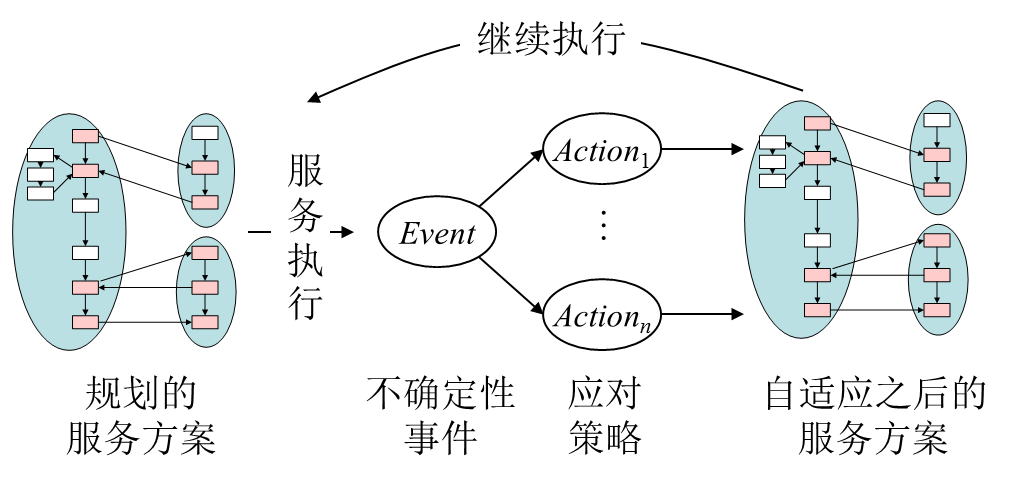
\includegraphics[width = 0.5\textwidth]{uc_plan}
\caption{按需应变的服务不确定性自适应决策}\label{uc_plan}
\vspace{-1em}
\end{figure}

为了应对不确定性,核心策略就是“按需应变”:根据预期发生的或已经发生的不确定性,对服务做出调整。这里的“变”即各种不确定性事件,“应”即所采取的对策,而“需”则是指在决定采取何种对策时应考虑客户/提供者的特征。按需应变的目标是:以最小的代价,使不确定造成的损失最小化。由于不确定性的动态性,所采取的应对策略也不可能是提前计划好的静态策略,需要根据服务执行时的具体情况选取最优的应对策略。

因此,对服务不确定性进行分析和建模,在服务执行时出现不确定性时以最小的代价将服务恢复至正常状态,并且使得此正常状态后得以成功执行的价值最高,这将避免在服务出现不确定情况时而临时采取对策而造成过高的代价,从而提升顾客满意度。

%本文根据服务执行中发生的具体不确定性,利用不确定性触发关系图(UTG)刻画不确定性事件所导致的服务状态以及所采取的决策动作之间的转换关系,以服务成功执行的概率最大、时间延迟最小、成本最低作为决策优化的目标,建立基于Markov 决策过程(MDP) 的不确定性优化决策模型并加以求解,生成对当前服务方案的最优改进策略。

% !Mode:: "TeX:UTF-8" 
\section{国内外在该方向的研究现状及分析}
\subsection{国外研究现状}

“不确定性”和“风险”是各个学术领域均比较关注的一个研究问题。本节简要归纳不确定性的分类、度量和各类不同的处理对策,思路如图~\ref{uc_ways}~所示。

\begin{figure}[htbp]
\centering
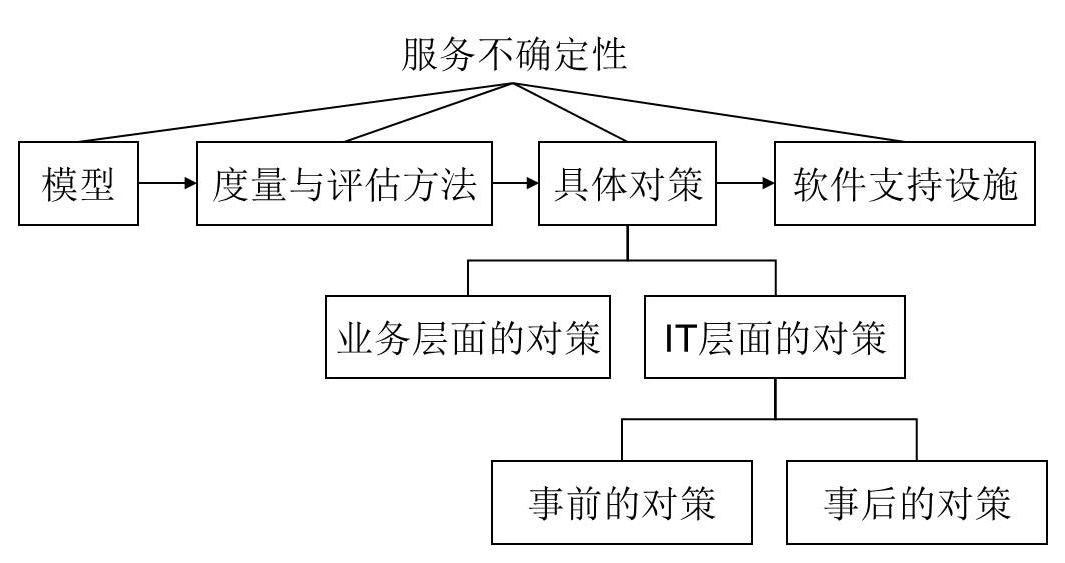
\includegraphics[width = 0.4\textwidth]{uc_ways}
\caption{按需应变的服务不确定性自适应决策}\label{uc_ways}
\vspace{-1em}
\end{figure}

在按需服务环境中,服务执行之前供需双方在性能、可靠性和可用性等~QoS~方面达成服务级别协议~(SLA)~。目前得以广泛应用的~Web Service Level Agreement (WSLA)~是一种用于定义和监测~web~服务的~SLA~描述语言和框架\citeup{keller2003wsla},为~SLA~的建模、扩展、度量和监控提供支持。文献\cite{kokash2007evaluating}\cite{chan2009fault}\cite{ardagna2006faults}对服务运行时可能发生的不确定性进行了不同角度的分类,从不确定性发生的层次(应用层面、服务层面、基础设施/中间件层面)、不确定性发生时的表现(服务/数据缺失、非期望的服务行为、性能问题、协议违反)等方面阐述了不确定性的含义,通过基于SLA的风险度量与估算方法协助发现不确定性及其影响\citeup{michalk2010risk}。

服务不确定性与其可靠性息息相关,因此可采用可靠性保障的方法来解决~web~服务中的不确定性问题\citeup{subramanian2008enhancement},在最初构建服务方案时就考虑可能面临的风险,将可靠性、不确定性等因素加入到服务选择与服务组合模型/算法中,以降低未来执行中的风险。使用随机~Petri~网等工具对~web~服务组合方案进行建模并计算其可靠性\citeup{zhong2008reliability},或者将服务发生风险时的依赖关系作为服务组合的可靠性优化依据\citeup{liu2009risk},通过~Markov~决策过程(MDP)等方法来选择最符合客户风险偏好的可靠服务\citeup{harney2008selective}\citeup{gao2011reliability}。

为了在服务执行产生不确定事件时能够通过恢复机制来保障可靠性\citeup{chan2009design},可基于冗余策略预先配置备用服务或多个替代配置方案(配置树、执行计划)来提升服务方案的容错能力\citeup{kokash2006service},目标是使服务方案具备自我治愈的能力\citeup{ardagna2006faults}。当现有服务无法正常执行时直接由备选服务接替执行,也可采用备选流程的方式,在当前流程出现问题时直接切换到备选流程。为此需在服务建模阶段考虑各种不确定性,对建模元素的实现机制和应用场景进行扩展以提高模型描述能力和适应性\citeup{fan2002service}。

\subsection{国内研究现状}

服务执行过程中的典型动态自适应策略包括:服务替换、服务重组等服务重配置方法、恢复与补偿机制等策略\citeup{erradi2006recovery}。服务替换考虑服务的功能和非功能特性,基于服务的参数类型等静态属性和动态行为特性的匹配保证替换前后服务过程功能的一致性,基于客户的QoS偏好对服务效用进行度量来保证和优化替换后的服务质量\citeup{athanasopoulos2009service},并引入context对服务的可替换性进行判断\citeup{pathak2007context}。

服务重组分为服务的大规模重选取和服务路径的重规划。文献\cite{bouhini2010discovery}使用服务片段作为重规划的基本单元以提升效率,文献\cite{bucchiarone2010design}提出了一组系统化的原则和指南,指导设计者如何构造/重规划适应变化的服务。为降低重组代价,对服务过程内处于不同执行状态的部分进行划分,每次尝试都期望在尽量小范围内弥补不确定性产生的后果,并在尝试失败后逐渐扩大重组范围\citeup{zhai2009soa}。还可使用修补技术对当前服务组合方案进行改变和增强,使之适应各类故障\citeup{yan2010self}。还可根据服务执行反馈的状况,采用进行持续规划\citeup{kaldeli2011continual},以适应执行过程中出现的各类不确定情况。

\subsection{国内外文献综述的简析}
如上所述,目前关于服务不确定性的研究已经有了丰富的研究,但尚显不足。

(1)~大部分研究者站在软件服务的开发、运行和维护的角度上,探讨“当某服务执行出现异常”之前或之后如何应对。而本课题站在客户或者中介方的角度,他们作为服务的使用者,不可能也无需了解软件服务的内部执行细节,只是从外部观测到各类异常的发生,而无法得知造成异常的原因(例如服务器内部出错、网络出错等)。在这种情况下,通过各类不确定性的决策方法,提高第三方服务中介所构造的整体服务方案适应不确定性的能力,是本课题的研究重点,也是区别于传统研究的观点之一。

针对此类问题,归纳起来,目前的研究主要分为两类:
a)~建模阶段对服务模型进行抗风险能力的增强,一旦运行时发现问题即可按预案进行应对;
b)~运行阶段对相关服务进行替换、重组或修补,并确保操作前后服务功能和QoS的一致性。
尚有以下两点不足:
a)~关注替换、重组、修补等单一决策动作如何操作、如何实施,对哪种动作的效果最优的考虑显得不足;
b)~决策目标定位在服务功能的相容性和~QoS~的可保障性,较少从经济角度考虑不确定性带来的时间和成本方面的损失。本文尝试着从这两点入手展开研究,试图将服务层面的不确定性与业务层目标结合起来,寻求处理不确定性的最优决策动作。

(2)~目前的研究通常将~business~和~IT~层面的不确定性割裂开来,分别研究。例如,针对供应链中的需求/供给/制造的不确定性,研究业务层面如何应对;针对底层的~web service~和服务系统执行中的出错、延迟、失败等不确定性,研究软件层面如何应对。但是二者本质上是有联系的,将它们关联起来并建立映射,是本课题的另一个观点。

针对此类问题,目前的研究主要是针对不同的业务情况采取不同的方法,其不足体现在两个方面,a)~没有对业务的不确定性进行系统化的分类处理,以至于不确定性的处理方案没有重用性和对处理结果统一的价值度量;b)~完全停留在~business~层面纯手工进行决策,忽略了~IT~手段可以辅助业务不确定性的决策,效率低下并且无法准确量化不确定性的决策的代价;


% !Mode:: "TeX:UTF-8"
\section{主要研究内容}

本课题将将站在服务使用者的角度,研究软件服务和业务服务的不确定性决策,首先建立服务不确定性决策模型,基于此模型采用软件服务实现不确定性决策,然后上升到业务服务的不确定性决策。通过对软件服务的不确定性仿真,进而将业务服务的不确定性决策应用在海运物流的业务中,从而完成本课题。

因此,将要研究的内容主要分为~5~个部分,它们之间的逻辑关系如图~\ref{main_content}~所示。

\begin{figure}[htbp]
    \centering
    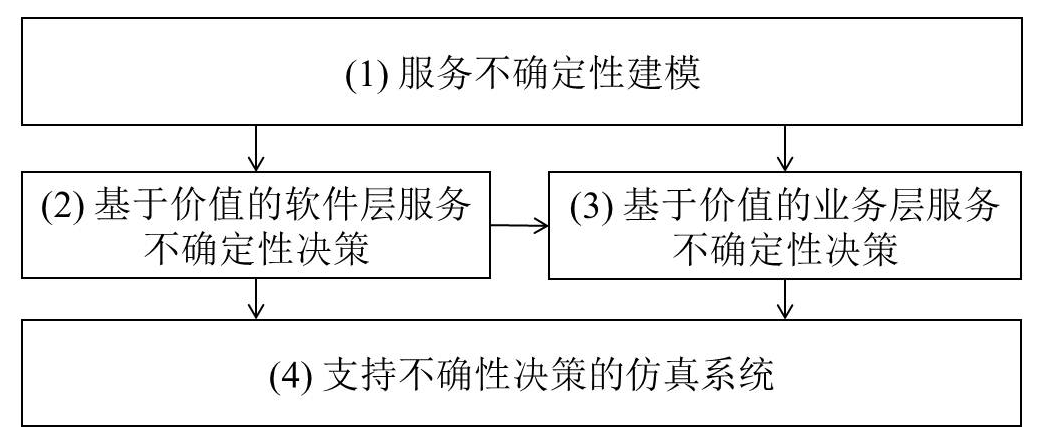
\includegraphics[width = 0.5\textwidth]{main_content}
    \caption{项目研究内容之间的逻辑关系}\label{main_content}
    \vspace{-1em}
\end{figure}

\setcounter{paragraph}{0}

\paragraph{基于价值的服务不确定性建模}

针对软件服务,分别识别服务执行过程中可能面临的多种不确定性,对服务不确定性进行分类,并提出不确定性触发关系图~(Uncertainty Triggering Graph, UTG)~以描述多种不确定性事件之间可能存在的触发关系。同时,识别每种不确定性事件发生后可能的决策动作并将其分类,由于采用不同的动作其所获得的价值是同的,因此建立其收益/成本度量模型,来衡量不同决策动作之间的优劣,并研究决策出最优的动作。

\paragraph{MDP~的软件服务不确定性决策}

根据服务执行中发生的具体不确定性,研究相应的不确定性触发关系图~(UTG)~的动态生成方法。提出基于动态~UTG~的不确定性影响范围及代价分析方法。识别优化目标(服务成功概率最大、时间延迟最小、成本最低),建立基于~Markov~决策过程~(MDP)~的不确定性优化决策模型并加以求解,生成对当前服务方案的最优改进策略。研究面向最小代价的运行时服务流程重组算法。

\paragraph{基于~A*~搜索的业务服务不确定性决策}

在业务层面,有比软件层面更灵活的需求和变化多端的外部环境。根据业务的不确定性,抽象出业务层面不确定性事件的通用特征,识别优化目标(服务执行成功的概率最大、服务执行时间最接近顾客期望时间、成本最低),建立业务层面服务不确定性的通用模型,采用~A*~算法对已出现故障的服务流程搜索最优的恢复策略。

\paragraph{不确性决策的仿真系统}

针对软件层面的服务不确定性,开发一个服务不确定性决策原型系统。此系统将融入基于~Markov~决策过程的服务不确定性决策方法,将不确定性事件采用某种随机策略产生,使得服务执行至故障状态,采用不确定性决策算法对故障状态的服务流程进行最优动作的决策,使得服务方案得以继续执行。

针对服务不确定性算法(基于~MDP~的服务自适应算法),采用传统的单步决策(贪心决策)与之进行对比,通过对比本课题的算法和传统算法的价值差(价值衡量),以及算法本身(时间复杂度和空间复杂度),从而证明本课题算法的有效性。

\paragraph{不确性决策在海运物流中的应用验证}

针对业务层面的服务,在以上两个软件层面的不确定性决策研究的基础之上,通过具体的海运业务示例,建立海运业务的不确定性的分类,研究针对其具体业务的决策方法,以及其不确定性事件之间可能存在的触发关系,建立其服务不确定性决策模型,并自动求解其针对当前业务执行状态的最优(成本最低/价值最高)策略。

针对业务层面的不确定性,通过海运业务示例,提供海运服务接口和产生海运不确定性事件,对比其决策结果与传统人工决策结果,并对比其自动化决策效率和传统的人工决策效率之间的差值,将证明其决策效果的有效性和自动化决策的高效性。

针对海运物流业务层面,开发一个具备海运物流不确定性事件自动化决策的应用系统。此系统将建立海运业务的具体业务执行流程,用~Web Service~提供海运业务的服务接口,从而使得海运业务IT化。系统将采用服务不确定性决策算法,针对业务层面进行服务不确定性决策,使之具备海运业务不确定性的自动决策功能。

% !Mode:: "TeX:UTF-8"
\section{研究方案及进度安排}

\subsection{研究方案}

本课题将要研究的内容主要分为~5~个部分,首先研究软件服务和业务服务的不确定性决策,建立服务不确定性决策模型,其次基于此模型采用软件服务实现不确定性决策,然后上升到业务服务的不确定性决策,最后通过对软件服务的不确定性仿真,再进而将业务服务的不确定性决策应用在海运物流的不确定性决策中。以下则是针对这五个方面的具体研究方案。

\subsubsection{基于价值的服务不确定性建模}
\setcounter{paragraph}{0}
\paragraph{服务方案}

使用服务流程表示当前执行中的服务方案,表示为如式(\ref{equation:splan})所示。
\begin{equation}\label{equation:splan}
SPlan = \left( {A,E,fc,dc} \right)
\end{equation}
\begin{tabularx}{\textwidth}{@{}l@{\quad}l@{\pozhehao }X@{}}
    式中
    & ${A}$ & 活动集合,表示为~$\{{a_1}, {a_2},...,{a_n}\}$ ~; \\
    & ${E}$ & 活动之间的时序依赖关系,表示为~$\{{e_1}, {e_2},...,{e_n}\}$ ~;\\
    & ${fc}$ & 服务若执行失败,提供方需要支付给客户的补偿金;\\
    & ${dc}$ & 表示服务若执行延期,每单位时间延迟需要支付给客户的补偿金。
\end{tabularx}\vspace{\wordsep}

针对每个活动,可表示为如如式(\ref{equation:activity})所示。
\begin{equation}\label{equation:activity}
{a_i} = ({CS_i}, {S_{i0}}, {LST_i}, {LET_i})
\end{equation}
\begin{tabularx}{\textwidth}{@{}l@{\quad}l@{\pozhehao }X@{}}
    式中
    & ${CS_i}$ & 活动的可替换服务集;\\
    & ${S_{i0}}$ & 当前被选中用于执行该活动$i$的具体服务;\\
    & ${LST_i}$ & 最晚开始时间;\\
    & ${LET_i}$ & 最晚结束时间;
\end{tabularx}\vspace{\wordsep}

针对活动之间的依赖关系,一般的服务流程中存在各种复杂结构关系\citeup{jaeger2004qos},本文考虑串行与并行两种关系,并使用如式(\ref{equation:e})表示,其意义是活动${a_j}$需要在活动${a_i}$执行完成后才能开始执行,在~DAG~图中体现的则是从结点${a_i}$到结点${a_j}$之间有一条有向边。
\begin{equation}\label{equation:e}
e = ({a_i},{a_j})
\end{equation}

对于候选服务,是以服务编号和~QoS~组成的二元组,如式(~\ref{equation:cs}~)所示。其QoS是以执行时间~$t$~、价格~$p$~,可靠性~$r$~组成的三元组,如式(~\ref{equation:qos}~)所示。

\begin{equation}\label{equation:cs}
CS = (id, QoS)
\end{equation}

\begin{equation}\label{equation:qos}
QoS = (t, p, r)
\end{equation}

\paragraph{不确定性事件} \label{sec:uc_event}

本课题关注的是服务执行过程中从外界可观测到的事件,即站在服务使用者的角度观察系统的运行状态,而不关心服务执行环境内部是何种原因而产生的事件。这样做的原因是服务方案通常是由服务中介方负责构建的,方案中使用的各服务并不受其控制,故只能从外部观察。

事件可表示为如式(\ref{equation:event})所示,其中t为事件发生的时刻,a为事件所涉及的活动,EType表示事件的类型。
\begin{equation}\label{equation:event}
event = (t, a, EType)
\end{equation}
\begin{tabularx}{\textwidth}{@{}l@{\quad}l@{\pozhehao }X@{}}
    式中
    & $t$ & 事件发生的时刻;\\
    & $a$ & 事件所涉及的活动;\\
    & $Type$ &事件的类型。
\end{tabularx}\vspace{\wordsep}

考虑事件的类型~$EType$~。服务执行过程中的产生的事件分为两大类:正常事件、不确定性事件。前者是一项活动按计划正常开始和正常执行结束时所发出,后者是指活动未按预期开始或结束,或者执行失败。按照事件触发的机制,可分为以下三类:

\begin{itemize}
    \item 由定时器所触发的事件,表示某活动未在期望时间点上开始执行或执行完成。服务执行引擎根据服务方案中为每个活动预设的最晚开始和最晚结束时刻对服务执行进行监控,如果到达~$LST_i$~或~$LET_i$~时刻活动未能开始或结束,将发出以下两类事件:
    
    $E_{01}$:~活动~$a_i$~在当前时刻~$t$~未开始执行,满足~$t>LST_i+\delta$~ (~$\delta$~是一个足够小的时间间隔),一旦系统在~$LST_i+\delta$~时刻未发现~$a_i$~开始执行,则发出该类事件;
    
    $E_{02}$:~与之类似,活动~$a_i$~在当前时刻~$t$~未按计划执行结束,满足~$t>LETi+\delta$~;
    
    \item 由活动的开始执行所触发的事件。一旦服务活动开始执行,系统即产生该类事件。
    
    $E_{11}$:~活动准时/提前开始,此时~$t\le LST_i$~。
    
    $E_{12}$:~活动延迟开始,此时~$t>LST_i$~。
    
    \item 由活动执行结束所触发的事件,可分为以下两种情况:
    
    $E_{21}$:~活动执行失败或错误,未得到期望结果;
    
    $E_{22}$:~活动执行成功。~$t\le LET_i$~表示活动提前或准时执行结束,而~$t>LETi$~表示活动有延迟。
    
\end{itemize}

\paragraph{服务执行的状态} \label{sec:service_state}

服务流程在执行过程中产生各种正常或不确定事件,导致服务执行不确定状态。本节给出服务执行状态的刻画。

a)~单个服务的状态

首先定义活动的状态。对某活动~$a_i$~,其状态可表示为如式(\ref{equation:state})所示。

\begin{equation}\label{equation:state}
state(a_i)=STATE\_TYPE^{N/U}<T, C>
\end{equation}
\begin{tabularx}{\textwidth}{@{}l@{\quad}l@{\pozhehao }X@{}}
    式中
    & $T$ & 处于当前状态时相比于预期服务方案的时间延迟~(TimeDelay)~;\\
    & $C$ & 处于当前状态时相比于预期服务方案的成本溢出~(CostOverflow)~;\\
    & $N$ & 该状态为正常状态~(Normal)~,即时间和成本未超出初始服务方案中对~$a_i$~的时间与成本的规划~$(T\le 0, C\le 0)$~;\\
    & $U$ & 该状态为不正常状态~(Uncertain)~,即当前存在时间延迟或者成本溢出~$(T>0, C>0)$~;
\end{tabularx}\vspace{\wordsep}

式(\ref{equation:state})可简写为~$STATE\_TYPE^{N/U}$~。~$STATE\_TYPE$~可为以下6种类型之一,对~$NOT\_READY$~、~$FAIL$~、~$CANCEL$~三类状态来说,不存在正常或不正常的分类,可不需标注上标~$N$~或~$U$~。

\begin{itemize}
    
    \item ~($NOT\_READY$):~$a_i$~至少有一个前序活动尚未执行结束,故~$a_i$~尚无开始执行的条件,即~$\exists a' \in \{ {a_j}|\exists e = ( {{a_j},{a_i}} )\} ,state ( {a'} ) \ne FINISH \Rightarrow state ( {{a_i}} ) = NOT\_READY$~。这是所有活动的缺省状态。
    
    \item 待执行($READY$):~若~$a_i$~的所有前序活动均已执行完毕(处于~$FINISH$~状态),且对这些活动的决策动作均非“终止”时,ai具备了执行的先决条件,进入该状态,即~$\forall a' \in \{ {a_j}|\exists e = ( {{a_j},{a_i}} )\} ,state ( {a'} ) = FINISH \wedge Action(a') \ne STOP \Rightarrow state ( {{a_i}} ) = READY$~。当~$a_i$~处于READY状态且产生~$E_{01}$~时,它仍然处于~$READY$~状态;
    
    \item 执行中($EXEC$):~当本活动产生~$E_{11}$~、~$E_{02}$~事件时,~$a_i$~正在执行中,但尚未结束;
    
    \item 执行后失败($FAIL$):~本活动产生~$E_{21}$~事件,~$a_i$~执行结束,但未得到期望输出,执行失败;
    
    \item 执行后成功~($FINISH$):~本活动产生~$E_{22}$~事件,~$a_i$~执行结束,已得到期望结果;
    
    \item 取消~($CANCEL$):~当某活动处于~$READYU$~、~$FINISHU$~或~$FAIL$~状态,并且决策动作将该活动终止时,~$a_i$~被人为取消,服务方案停止执行而完全失败。
\end{itemize}

事件或决策动作导致活动的状态变化,状态之间的转换关系如图~\ref{figure:state_trans}~所示。
\begin{figure}[htbp]
    \centering
    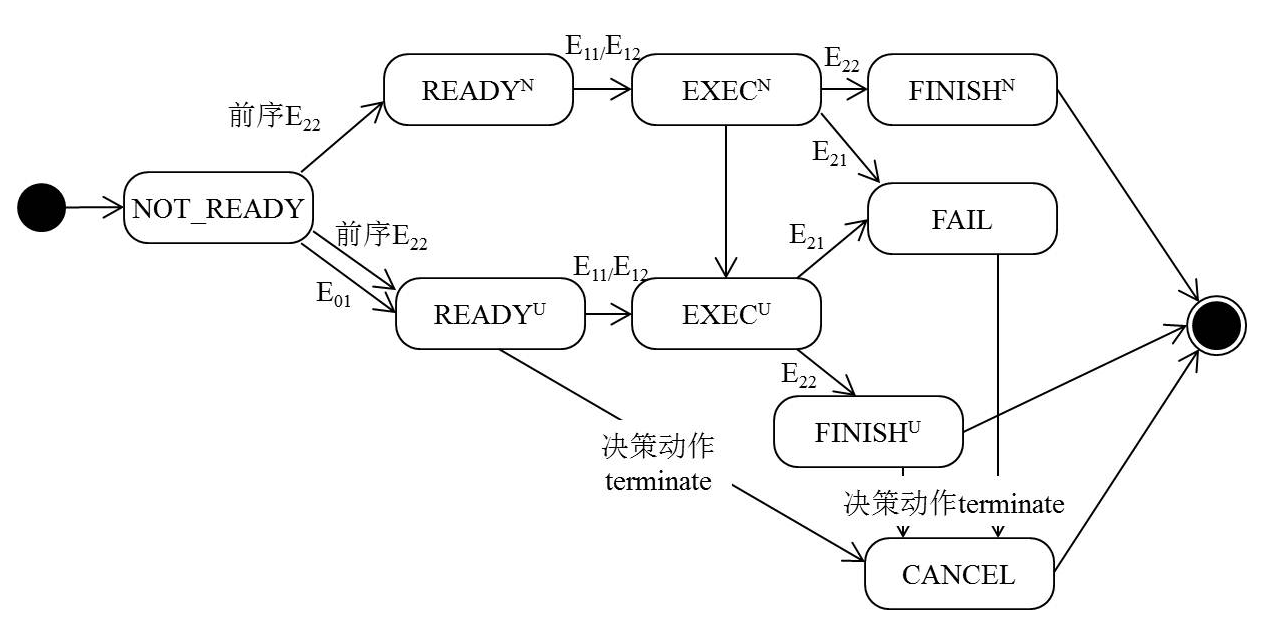
\includegraphics[width = 0.6\textwidth]{state_trans}
    \caption{服务活动的状态转换关系}\label{figure:state_trans}
    \vspace{-1em}
\end{figure}

b)~服务执行的整体状态

将服务执行“前锋线”~(forward line)~上的各服务活动的状态联合起来,共同表示服务执行的整体状态~state(SPlan)~,如式(\ref{equation:state_total})所示。

\begin{equation}\label{equation:state_total}
state = < state(a_i),state(a_{i+1}),..., state(a_j)>
\end{equation}
\begin{tabularx}{\textwidth}{@{}l@{\quad}l@{\pozhehao }X@{}}
    式中
    & $state(a_i)$ & 活动~$a_i$~的状态。
\end{tabularx}\vspace{\wordsep}

所谓的“前锋线”~(Front Line)~,是指将已经执行的部分和尚未执行的部分分开的一条线,表示为~$FL(SPlan)=\{(a_i, state(a_i))\}$~,它由一组活动及其状态构成,~$prodecessor(FL)$~、~$successor(FL)$~分别为其左侧和右侧的活动集合。处于~$FL$~中的每一个服务,可能是~$READY^{N/U}$~、~$EXEC^{N/U}$~、~$FAIL$~、~$FINISH^{N/U}$~的某一状态,其所有前序活动的状态必须是~$FINISH^{N/U}$~,其所有后序活动的状态必须是~$NOT\_READY$~,即
$\forall {a_i} \in FL,state({a_i}) \in \{ READ{Y^{N/U}},{\rm{ }}EXE{C^{N/U}},{\rm{ }}FAIL,{\rm{ }}FINIS{H^{N/U}}\} ;\forall a' \in predecessor(FL),state(a') = FINIS{H^{N/U}};\forall a' \in successor(FL),state(a') = NOT\_READY.$

例如,在某一时刻服务执行状态如图~\ref{figure:front_line}~所示,虚线表示流程执行的前锋线,它左侧的活动~$(a_1, a_2, a_5)$~均处于~$FINISH$~状态,它右侧的活动~$(a_7, a_8, a_9)$~均处于~$NOT\_READY$~状态,而在线上的三个活动~$(a_3, a_4, a_6)$~,分别处于~$READY$~、~$EXEC$~、~$FAIL$~状态。

\begin{figure}[htbp]
    \centering
    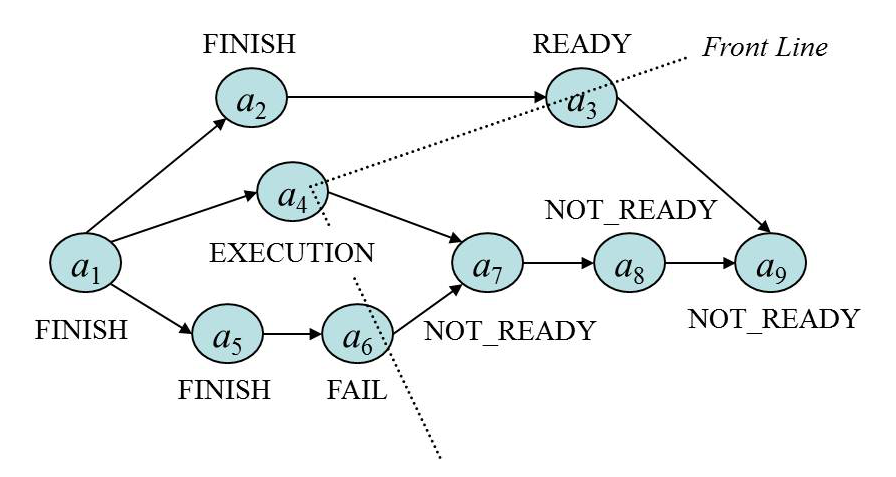
\includegraphics[width = 0.5\textwidth]{front_line}
    \caption{服务方案执行中的状态划分与前锋线}\label{figure:front_line}
    \vspace{-1em}
\end{figure}

~$state(SPlan)$~可分为几类:
\begin{itemize}
    \item 执行前: ~$predecessor(FL) = \emptyset ,$ 对 $ \forall {a_i} \in FL,state({a_i}) = READ{Y^N}$~;
    \item 执行中: ~$FL \ne \emptyset ,predecessor(FL) \ne \emptyset ,successor(FL) \ne \emptyset $~;
    \item 执行结束(成功): ~$FL = \emptyset ,successor(FL) = \emptyset ,$ 对 $\forall {a_i} \in predecessor(FL),state({a_i}) = FINIS{H^{N/U}}$~;
    \item 执行结束(失败): ~$FL \ne \emptyset ,$ 且 $\exists {a_i} \in FL,state({a_i}) = FAIL$~;
\end{itemize}

\paragraph{不确定性触发关系图~(UTG)~} \label{sec:utg}
不确定性本身蕴含着服务的一种状态(不正常状态),它是可以传播的,若不采取任何对策(不作为),任由某一不确定性蔓延下去,将会造成更严重的后果(成本溢出、时间延误、执行失败)。即使采取了某一种对策,弥补了某些潜在后果,但可能不会完全弥补,因此也会扩散。这里提出不确定性触发关系图~(Uncertainty Triggering Graph, UTG)~表达~UC~之间的触发关系。利用~UTG~来计算不确定性事件及决策动作所引发的直接和间接代价。

UTG可表示为包含两类节点和两类边的有向图~UTG = ~$(rs, SS, AS, TSA, TAS)$,其中:
\begin{itemize}
    \item ~$rs=(a_i, state_i)$~表示根状态,代表活动~$a_i$~处于~$state_i$~时所生成的UTG;
    \item ~$SS={ss}$~为状态节点集合,其中包含两类节点:第一类为原子状态~$ss=(a_j, state_j)$~,第二类为嵌套的~UTG~根结点,可扩展为一棵完整的~UTG~树;
    \item ~$AS={action}$~为决策动作节点的集合;
    \item ~$TSA=ss \to action$~表示状态节点到决策动作节点的有向边;
    \item ~$TAS=action \to ss$~表示决策动作节点到状态节点的有向边,它具有三个属性:~$tp$~(该状态转移的概率)、~$\Delta T$~(该状态转移所造成的时间延迟)、~$\Delta C$~(该状态转移所造成的成本增加)。
\end{itemize}

如图~\ref{figure:utg_tree}~给出了~UTG~示意图,其中菱形框表示根状态,圆形节点表示原子状态,矩形框表示决策动作节点,箭头表示~$TSA$~和~$TAS$~。

\begin{figure}[htbp]
    \centering
    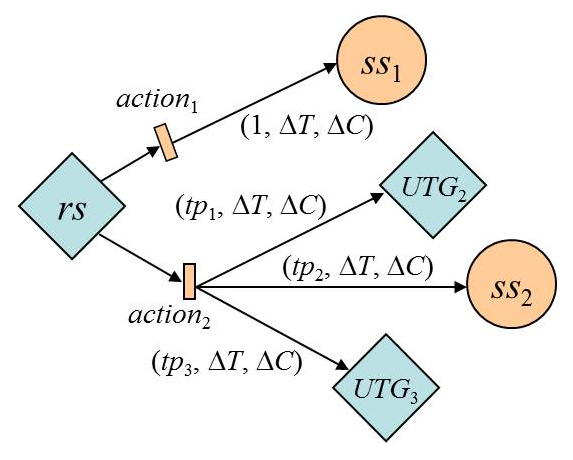
\includegraphics[width = 0.3\textwidth]{utg_tree}
    \caption{不确定性事件触发关系图~(UTG)~}\label{figure:utg_tree}
    \vspace{-1em}
\end{figure}

在~UTG~模型中,状态节点可以是一棵~UTG~的根节点,这代表了不同~UTG~之间的连接(不同活动的不确定性状态之间的转换)。若将此类~UTG~节点展开,即可形成如图~\ref{figure:many_utg_tree}~所示的形态。

\begin{figure}[htbp]
    \centering
    \includegraphics[width = 0.5\textwidth]{many_utg_tree}
    \caption{多棵UTG的连接~(UTG)~}\label{figure:many_utg_tree}
    \vspace{-1em}
\end{figure}

如图~\ref{figure:utg_example}~给出一个小例子。假设服务方案是由三个活动~$(a_1, a_2, a_3)$~串行构成的流程,图~(a)~表示活动~$a_1$~在~$READY^U$~状态下的~UTG~,~(b)~表示活动~$a_1$~在~$FINISH^U$~状态下的~UTG~,~(c)~表示~$a_1$~在~$FAIL$~状态下的~UTG~。

\begin{figure}[htbp]
    \centering
    \includegraphics[width = 0.5\textwidth]{utg_example}
    \caption{~UTG~的三个例子}\label{figure:utg_example}
    \vspace{-1em}
\end{figure}

~UTG~的结构与服务方案的流程结构密切相关。当出现不确定性事件之后,更新相关活动、状态和前锋线的信息,进而根据表~\ref{table:state_action}~的相关信息生成~UTG~。

\paragraph{决策收益(价值)} \label{sec:reward_section}

各种动作的目标是“使不确定性造成的损失尽可能小”,但并不保证服务一定能够从异常状态完全回到正常轨道,因此需要分析每种决策对服务执行的影响,计算其损失/受益,以此作为优化决策的依据。

决策动作对原有的服务方案进行了调整,对它的收益度量从以下三个因素入手:

\begin{itemize}

\item 使服务可以继续向后执行的概率考虑服务执行失败的赔偿~$fc$~。一般情况下服务失败后需支付给顾客的补偿较高,因此决策动作应尽可能保证服务可以继续执行下去。除了补偿上的考虑之外,还考虑到服务执行失败可能造成的客户流失。设决策动作之后,受影响的活动(可能为当前活动,也可能为下一步活动)执行成功的概率为~$r$~,那么该部分代价是~$(1-r) \times fc$~。

\item 若造成时间延迟而需支付的延误成本。设延误时间为~$\Delta T$~,那么该部分的代价是~$\Delta T \times dc$~。

\item 所引入的新成本~$\Delta C$. 对出现故障的服务进行恢复,势必会带来额外的服务成本,例如原来的服务不可用后替换为一个新的服务,而这个新的服务的价格即是引入的新成本。

\end{itemize}

因此,在当前状态下state采取决策动作action所带来的总收益如式(\ref{equation:reward})所示。

\begin{equation}\label{equation:reward}
Reward =  - ((1 - r) \times fc + \Delta T \times dc + \Delta C)
\end{equation}

面向不确定性的优化决策的目标可表述为:以最小的时间延迟和成本溢出,使服务可最大概率的进入到“成功结束”状态。

\subsubsection{基于~MDP~的软件服务不确定性决策}
\setcounter{paragraph}{0}
\paragraph{决策动作} \label{sec:action}

针对每一种不确定性,有多种可用的决策动作,需要识别出可能的决策动作,对其分类,并估算“若采取某项决策动作,可能会付出的直接/间接成本,以及对服务预期收益的影响”。将每一次决策表示为四元组~$SPlan,{a_i},state,action,SPlan'$~,含义是:当前服务执行方案~$SPlan$~,出现了不确定性事件导致某服务活动~$a_j$~进入状态~$state_j$~,此时采取对策~$action$~,得到新的方案~$SPlan'$~。

课题拟将决策动作归纳为五类:
\begin{enumerate}
    \item 终止~(terminate):~停止活动的执行,~$state(a_i)=FAIL$~,客户需求无法满足,服务失败,~$SPlan'=\emptyset $~;
    \item 不作为~(continue):~不做额外的调整对策,继续按原方案执行下去,~$SPlan'=SPlan$~;
    \item 重试~(retry):~重新执行出现异常的活动,即令~$state(a_i)=EXECU(T, C)$~;
    \item 替换~(substitute):~为出现异常的活动~$a_i$~从其候选服务集~$CS_i$~中选择一个新服务~$S_{ij}$~替换原服务~$S_{i0}$~,并重新启动执行~$a_i$~,即:~${S_i}_0 \leftarrow {S_{ik}}$~,其中~${S_{ik}} \in C{S_i}$~;
    \item 重组~(recompose):~对当前前锋线的右侧尚未执行的服务活动进行重组,形成替代方案并启动执行。这相当于对多个服务要素进行替换操作。即:将多个服务~${S_i}_0,{S_{i + 1,0}}, \ldots ,{S_j}_0$~分别替换为~${S_i}_k,{S_{i + 1,k}}, \ldots ,{S_j}_k$~, 其中~${S_i}_k \in C{S_i},{S_{i + 1,k}} \in C{S_{i + 1}}, \ldots ,{S_j}_k \in C{S_j}$~。
\end{enumerate}

终止、不作为和重试对服务方案的结构无影响,替换相当于为某一活动进行服务选择,重组相当于对后续未执行服务流程进行服务重组。替换和重组是为尚未执行的一个或多个活动选择时间更短或价格更低的候选服务,以此来消除之前因为不确定事件所导致的时间延误或成本溢出,替换可相当于对1个活动进行重新选择和组合服务,而在工作流不变的情况下的重组相当于对多个活动进行替换和组合服务。在此之前,需要根据~$SPlan$~的当前状态动态生成替换和重组的目标函数,使得当前造成的时间延误和成本溢出将最大程度的降低。

\paragraph{事件、决策和状态之间的关系}

在服务方案执行过程中,某时刻若产生某一不确定性事件,则会导致某一活动状态发生变化(若是正常事件,也可能不发生变化)。此时进行决策,根据决策动作修正服务方案并更新受影响的活动状态,继续投入执行。如此循环往复,直到服务停止或者执行成功。对活动执行前、执行后的状态,一旦该状态产生,马上进行决策;对活动执行中的状态,等活动达到执行后的某一状态时再进行决策。

需要说明的是,虽然决策针对服务的整体状态,但是每次动作只针对前锋线上的某一个活动进行。若前锋线上多个活动均处于异常状态,那么多个导致异常状态的事件必然是有先后次序到达的,因而决策也会随事件到达的先后次序进行。因此,决策只需要针对单一活动的状态进行,不需要针对多个异常活动进行。

针对服务所处的不同状态,可能采取的决策动作是上述五类中的子集。表~\ref{table:state_action}~的前四列给出了某一活动处于不同状态时可能采用的决策动作集合,以及决策之后可能导致的新状态。

% Table generated by Excel2LaTeX from sheet 'Sheet9'
\begin{table}[htbp]
    \caption{服务状态与决策动作之间的关系(软件层面)}
    \vspace{-0.5em}\label{table:state_action}\centering\zihao{5}
    \begin{threeparttable}
        \begin{tabular}{llllllll}
            %    \begin{tabularx}{\textwidth}{llXlllll}
            \toprule
            % Header
            \multicolumn{1}{|c|}{} 
            & \multicolumn{1}{c}{状态类型\tnote{1}} 
            & \multicolumn{1}{|c}{{决策动作}} 
            & \multicolumn{1}{|c}{决策后可能状态\tnote{1}} 
            & \multicolumn{1}{|c}{$r$~\tnote{2}} 
            & \multicolumn{1}{|c}{$\Delta T$} 
            & \multicolumn{1}{|c|}{$\Delta C$} \\
            \hline
            
            %Line 1
            \multicolumn{1}{|c|}{\multirow{9}{*}{\parbox{1em}{活动执行前的状态}}} 
            & \multirow{7}{*}{$READY^U$} 
            & \multicolumn{1}{|c}{{终止}} 
            & \multicolumn{1}{|l}{$STOP$} 
            & \multicolumn{1}{|c}{0} 
            & \multicolumn{1}{|c}{0} 
            & \multicolumn{1}{|c|}{$fc$} \\
            \cline{3-7}
            
            %Line 2
            \multicolumn{1}{|c|}{} 
            &       
            & \multicolumn{1}{|c}{\multirow{2}{*}{{不作为}}} 
            & \multicolumn{1}{|l}{$FINISH^{N/U}$} 
            & \multicolumn{1}{|c}{$R_{i0}$} 
            & \multicolumn{1}{|c}{\multirow{2}{*}{0}} 
            & \multicolumn{1}{|c|}{\multirow{2}{*}{0}} \\
            %        \cline{4-5}
            
            %Line 3
            \multicolumn{1}{|c|}{} 
            &       
            & \multicolumn{1}{|c}{} 
            & \multicolumn{1}{|l}{$FAIL$} 
            & \multicolumn{1}{|c}{0}
            & \multicolumn{1}{|c}{} 
            & \multicolumn{1}{|c|}{} \\
            \cline{3-7}
            
            %Line 4
            \multicolumn{1}{|c|}{} 
            &       
            & \multicolumn{1}{|c}{\multirow{2}{*}{替换}} 
            & \multicolumn{1}{|l}{$FINISH^{N/U}$} 
            & \multicolumn{1}{|c}{$R_{ik}\tnote{3}$} 
            & \multicolumn{1}{|c}{\multirow{2}{*}{$T_{ik}-T_{i0}$}} 
            & \multicolumn{1}{|c|}{\multirow{2}{*}{$C_{ik}-C_{i0}$}} \\
            %        \cline{4-5}
            
            %Line 5
            \multicolumn{1}{|c|}{} 
            &       
            & \multicolumn{1}{|c}{} 
            & \multicolumn{1}{|l}{$FAIL$} 
            & \multicolumn{1}{|c}{0} 
            & \multicolumn{1}{|c}{} 
            & \multicolumn{1}{|c|}{} \\
            \cline{3-7}
            
            %Line 6
            \multicolumn{1}{|c|}{} 
            &       
            & \multicolumn{1}{|c}{\multirow{2}{*}{重组}} 
            & \multicolumn{1}{|l}{$FINISH^{N/U}$} 
            & \multicolumn{1}{|c}{$R_{ik}\tnote{3}$} 
            %        & \multirow{2}{*}{$\sum\limits_{x = i}^j {({T_{xk}} - {T_{x0}})} $} 
            & \multicolumn{1}{|c}{\multirow{2}{*}{$\sum\limits_{x = i}^j {({T_{xk}} - {T_{x0}})} $}}
            & \multicolumn{1}{|c|}{\multirow{2}{*}{$\sum\limits_{x = i}^j {({C_{xk}} - {C_{x0}})} $}} \\
            
            %Line 7
            \multicolumn{1}{|c|}{} 
            &       
            & \multicolumn{1}{|c}{} 
            & \multicolumn{1}{|l}{$FAIL$} 
            & \multicolumn{1}{|c}{0} 
            & \multicolumn{1}{|c}{}
            & \multicolumn{1}{|c|}{} \\
            \cline{2-7}
            
            %Line 8
            \multicolumn{1}{|c|}{} 
            & \multirow{2}{*}{$READY^N$} 
            & \multicolumn{1}{|c}{\multirow{2}{*}{无需决策}} 
            & \multicolumn{1}{|l}{$FINISH^{N/U}$} 
            & \multicolumn{1}{|c}{$R_{i0}$} 
            & \multicolumn{1}{|c}{\multirow{2}{*}{0}} 
            & \multicolumn{1}{|c|}{\multirow{2}{*}{0}} \\
            
            %Line 9
            \multicolumn{1}{|c|}{} 
            &       
            & \multicolumn{1}{|c}{} 
            & \multicolumn{1}{|l}{$FAIL$} 
            & \multicolumn{1}{|c}{0} 
            & \multicolumn{1}{|c}{} 
            & \multicolumn{1}{|c|}{} \\
            \cline{1-7}
            
            %Line 10
            \multicolumn{1}{|c|}{\multirow{11}{*}{\parbox{1em}{活动执行后的状态}}} 
            & \multirow{7}{*}{$FAIL$} 
            & \multicolumn{1}{|c}{终止} 
            & \multicolumn{1}{|l}{$STOP$} 
            & \multicolumn{1}{|c}{0} 
            & \multicolumn{1}{|c}{0} 
            & \multicolumn{1}{|c|}{$fc$} \\
            \cline{3-7}
            
            %Line 11
            \multicolumn{1}{|c|}{} 
            &       
            & \multicolumn{1}{|c}{\multirow{2}{*}{重试}} 
            & \multicolumn{1}{|l}{$FINISH^{N/U}$} 
            & \multicolumn{1}{|c}{$R_{i0}$} 
            & \multicolumn{1}{|c}{\multirow{2}{*}{$T_{i0}$}} 
            & \multicolumn{1}{|c|}{\multirow{2}{*}{$C_{i0}$}} \\
            
            %Line 12
            \multicolumn{1}{|c|}{} 
            &       
            & \multicolumn{1}{|c}{}
            & \multicolumn{1}{|l}{$FAIL$} 
            & \multicolumn{1}{|c}{0} 
            & \multicolumn{1}{|c}{}
            & \multicolumn{1}{|c|}{} \\
            \cline{3-7}
            
            %Line 13
            \multicolumn{1}{|c|}{} 
            &       
            & \multicolumn{1}{|c}{\multirow{2}{*}{替换}} 
            & \multicolumn{1}{|l}{$FINISH^{N/U}$} 
            & \multicolumn{1}{|c}{$R_{ik}\tnote{3}$} 
            & \multicolumn{1}{|c}{\multirow{2}{*}{${T_{ik}}$}} 
            & \multicolumn{1}{|c|}{\multirow{2}{*}{${C_{ik}}$}} \\
            
            %Line 14 
            \multicolumn{1}{|c|}{} 
            &       
            & \multicolumn{1}{|c}{} 
            & \multicolumn{1}{|l}{$FAIL$} 
            & \multicolumn{1}{|c}{0} 
            & \multicolumn{1}{|c}{} 
            & \multicolumn{1}{|c|}{} \\
            \cline{3-7}
            
            %Line 15
            \multicolumn{1}{|c|}{} 
            &       
            & \multicolumn{1}{|c}{\multirow{2}{*}{重组}} 
            & \multicolumn{1}{|l}{$FINISH^{N/U}$} 
            & \multicolumn{1}{|c}{$R_{ik}\tnote{3}$} 
            & \multicolumn{1}{|c}{\multirow{2}{*}{${T_{i0}} + \sum\limits_{x = i}^j {({T_{xk}} - {T_{x0}})} $}}
            & \multicolumn{1}{|c|}{\multirow{2}{*}{${C_{i0}} + \sum\limits_{x = i}^j {({C_{xk}} - {C_{x0}})} $}} \\
            %        & \multicolumn{1}{|c}{\multirow{2}{*}{$\begin{array}{l}
            %                \sum\limits_{x = i}^j {({T_{xk}} - {T_{x0}})} \\
            %                {\kern 10pt}  + {T_{i0}}
            %                \end{array}$}} 
            %        & \multicolumn{1}{|c}{\multirow{2}{*}{$\begin{array}{l}
            %                \sum\limits_{x = i}^j {({C_{xk}} - {C_{x0}})} \\
            %                {\kern 10pt}  + {C_{i0}}
            %                \end{array}$}}  \\
            
            %Line 16
            \multicolumn{1}{|c|}{} 
            &       
            & \multicolumn{1}{|c}{} 
            & \multicolumn{1}{|l}{$FAIL$} 
            & \multicolumn{1}{|c}{0} 
            & \multicolumn{1}{|c}{} 
            & \multicolumn{1}{|c|}{} \\
            \cline{2-7}
            
            %Line 17
            \multicolumn{1}{|c|}{} 
            & \multirow{3}{*}{$FINISH^U$} 
            & \multicolumn{1}{|c}{不作为} 
            & \multicolumn{1}{|l}{后续活动$READY^U$~\tnote{4}} 
            & \multicolumn{1}{|c}{1} 
            & \multicolumn{1}{|c}{0} 
            & \multicolumn{1}{|c|}{0} \\
            \cline{3-7}
            
            %Line 18
            \multicolumn{1}{|c|}{} 
            &       
            & \multicolumn{1}{|c}{终止} 
            & \multicolumn{1}{|l}{$STOP$} 
            & \multicolumn{1}{|c}{0} 
            & \multicolumn{1}{|c}{0} 
            & \multicolumn{1}{|c|}{$fc$} \\
            \cline{3-7}
            
            %Line 19
            \multicolumn{1}{|c|}{} 
            &       
            & \multicolumn{1}{|c}{重组} 
            & \multicolumn{1}{|l}{后续活动$READY^{N/U}$~\tnote{4}} 
            & \multicolumn{1}{|c}{1} 
            & \multicolumn{1}{|c}{$\sum\limits_{x = i}^j {({T_{xk}} - {T_{x0}})} $} 
            & \multicolumn{1}{|c|}{$\sum\limits_{x = i}^j {({C_{xk}} - {C_{x0}})} $}  \\
            \cline{2-7}
            
            %Line 20
            \multicolumn{1}{|c|}{} 
            & $FINISH^N$
            & \multicolumn{1}{|c}{无需决策} 
            & \multicolumn{1}{|l}{后续活动$READY^N$~\tnote{4}} 
            & \multicolumn{1}{|c}{1} 
            & \multicolumn{1}{|c}{0} 
            & \multicolumn{1}{|c|}{0} \\
            \bottomrule
            
            %            \multicolumn{7}{l}{[1] \textit{}}  \\
            %            \multicolumn{7}{l}{\textit{~~~~FINISH且不采用“终止”决策时才能够过渡到READY;}} \\
            %            \multicolumn{7}{l}{[2] \textit{$r$为决策后,服务可继续执行的概率; }}  \\
            %            \multicolumn{7}{l}{[3] \textit{$S_{ik}$为替换后的服务或者重组后最先执行的服务。 }}  \\
        \end{tabular}%
        \begin{tablenotes}
            \item[1] 决策动作前状态所带参数为$(T,C)$, 决策后状态参数变为~$(T+\Delta T, C+\Delta C)$,~ 其中~$\Delta T \ge 0$, ~$\Delta C \ge 0$~; 
            \item[2] $r$~为决策后,服务可继续执行的概率;
            \item[3] $S_{ik}$~为替换后的服务或者重组后最先执行的服务,~$R_{ik}$~为此服务的可靠性。
            \item[4] 是否可以过渡到后续活动的~$READY$~状态,取决于流程的结构,只有后续活动的所有前序活动均处于~$FINISH$~且不采用“终止”决策时才能够过渡到~$READY$;
        \end{tablenotes}
    \end{threeparttable}
\end{table}%

\paragraph{决策收益}

在基于~MDP~的软件服务不确定性决策方法中,根据~\ref{sec:reward_section}~节所述的几种决策收益的计算方案,得出如下基于~MDP~的服务不确定性决策收益的计算方式。
\begin{itemize}

\item 服务执行失败付给用户的赔偿为~$fc$~. 这是整体服务执行失败时的赔偿。

\item 若造成时间延迟而需支付的延误成本。设延误时间为~$\Delta T$~,那么该部分的代价是~$\Delta T \times dc$~。

\item 所引入的新成本~$\Delta C$。~对终止和不作为两种动作来说,新成本为0;对重试动作来说,新成本为重新支付的当前服务使用价格;对替换动作来说,新成本为所选新替代服务的使用价格;对重组动作来说,新成本为所选的多个替代服务的使用价格与原方案中相应服务的使用价格之差。

\end{itemize}

因此,在当前状态下state采取决策动作action所带来的总收益即可根据式(\ref{equation:reward})计算得出。

\paragraph{基于~MDP~的不确定性决策方法}

马尔科夫决策过程~(MDP)\citeup{liuke2004}~将马尔可夫过程与确定性的动态规划相结合,决策者周期或连续观察随机动态系统,序贯的做出决策,系统下一步的状态是随机的,并且其状态转移概率具有马尔可夫性。决策者根据新观察到的状态,再作新的决策,依此反复地进行。通过此种决策,使系统运行的全过程达到某种最优运行效果,选取控制系统发展的最优策略。

a)~{模型}

服务执行过程中面临的各种不确定性以及对其所做出的决策,符合~Markov~决策过程的定义。因此,采用基于~MDP~的方法进行服务自适应演化过程中的决策,根据当前服务执行状态、发生的不确定性事件、不确定性事件之间的触发关系~(UTG)~,考虑未来的收益和代价,做出当前不确定状态下的最优决策。

按照~MDP~的数学模型,需要首先建立决策时刻~$T$~、服务状态~$S$~、决策动作~$A$~、转移概率~$P$~、代价~$Reward$~的数学表达。
\begin{itemize}

\item 时刻~$T$~: 前服务环节执行中/执行后发生不确定事件、或者预知到尚未执行的环节将会发生不确定事件时开始决策,此时为时刻0。如图~\ref{figure:many_utg_tree}~所示的多棵~UTG~连接形成完全触发关系图,叶子结点的状态处于最终时刻~$V$~,“完全触发关系图”的层数是周期个数。这是一个不定周期的时刻序列。

\item 状态~$S$~: 服务前锋线上的所有活动的状态即可表示为服务流程的状态,原因是前锋线上的活动状态已知,则可知所有活动的状态。将服务流程的所有活动的六种状态组成一个状态集合,形成~MDP~状态~$state$~, 即~$state =  < state({a_1}),state({a_2}), \ldots ,state({a_n}) >$~,每个状态附着两个参数(~$T$~和~$C$~);

\item 动作~$A$~:共有终止、不作为、重试、替换、重组五个动作,不同状态下可执行的动作集合有所不同(见表~\ref{table:state_action}~)。

\item 转移概率~$P$~:转移概率由当前的决策动作和服务活动的状态联合决定,即~$p(state_j|state_i,action)$~的值有以下几类情况:
\begin{itemize}
    \item ~$1;~if~action = continue/terminate$~
    \item ~$reliability;~if~action = retry/substitute/re-compose~ \& ~ state_j = FINIS{H^{N/U}}$~
    \item ~$1 - reliability;~if~action = retry/substitute/re-compose ~\& ~ state_j = FAIL$~
\end{itemize}
其中~$reliability$~指的是将要执行的服务端可靠性,若有多个服务,则是多个服务可靠性之积。

\item 报酬函数~$Reward$~:在~\ref{sec:reward_section}~节中给出。

\end{itemize}

b)~{算法}

基于上述五个方面的基本定义,采用有限阶段向后递归迭代~MDP~算法进行最优决策序列的求解,得到对当前服务的决策动作。

算法:基于~MDP~的服务不确定性优化决策

输入:服务方案~$SPlan$~、与当前发生的不确定性事件相关的活动~$activity$~、
~$SPlan$~中各个活动的当前状态;

输出:最优马氏策略及其成本

步骤1~根据出现故障的活动~$a$~,按照表~\ref{table:state_action}~构造~UTG~,并将多棵~UTG~连接形成“完全触发关系图”,从而形成状态转移表;

步骤2~定义当前的不确定状态为时刻0,以此生成向后衍生的UTG,直至服务方案最后一个结点,此时为最终时刻V。从而生成0到~$V$~的~$V+1$~个时刻的若干个状态、若干个动作、相应的转移概率报酬;

步骤3~令~$t=V$~,且对所有~$V$~时刻的状态~$state_V \in S$~,令~${u_V}( {state_V} ) = Reward_V( {state_V} )$;

步骤4~如果~$t=0$~,则~$\pi  = (f_0,f_1,\ldots ,f_{V-1})$~为最优的马氏策略,而~${u_0}( state_0)$~为最优的值函数,算法停止。否则,令~$t=t–1$~,进入步骤5;

步骤5~对所有~$state_t \in S$~,计算

\begin{equation}\label{equation:backward_mdp}
\begin{array}{l}
{u_t}(stat{e_t}) = \mathop {\max }\limits_{action \in Action(stat{e_t})} \{ Rewar{d_t}(stat{e_t},action)\\
{\rm{                        }} + \sum\limits_{stat{e_{t + 1}} \in S} {{p_t}(stat{e_{t + 1}}|stat{e_t},action){u_{t + 1}}(stat{e_{t + 1}})} \} 
\end{array}
\end{equation}

并记集合

\begin{equation}\label{equation:backward_mdp_arg}
\begin{array}{l}
Actio{n_t}(stat{e_t}) = \mathop {\arg \max }\limits_{action \in Action(stat{e_t})} \{ Rewar{d_t}(stat{e_t},action)\\
{\rm{                       }} + \sum\limits_{stat{e_{t + 1}} \in S} {{p_t}(stat{e_{t + 1}}|stat{e_t},action){u_{t + 1}}(stat{e_{t + 1}})} \} 
\end{array}
\end{equation}

任意取~$f_t(state_t) \in Action_t(state_t)$~,于是定义了~$t$~时刻的决策规则~$f_t$~。而0时刻的决策~$f_0$~则是对当前故障时刻的故障状态采取最优的直接动作。

步骤6~返回步骤3。

\subsubsection{基于XX的业务服务不确定性决策}



\subsubsection{不确性决策的仿真系统}

针对服务不确定性,将开发出一个软件层面的不确定性原型系统,此系统将采用随机的不确定性事件产生器,将预定义的组合服务进行仿真过程,其原型系统结构如图~\ref{figure:prototype_system}~所示。

\begin{figure}[htbp]
    \centering
    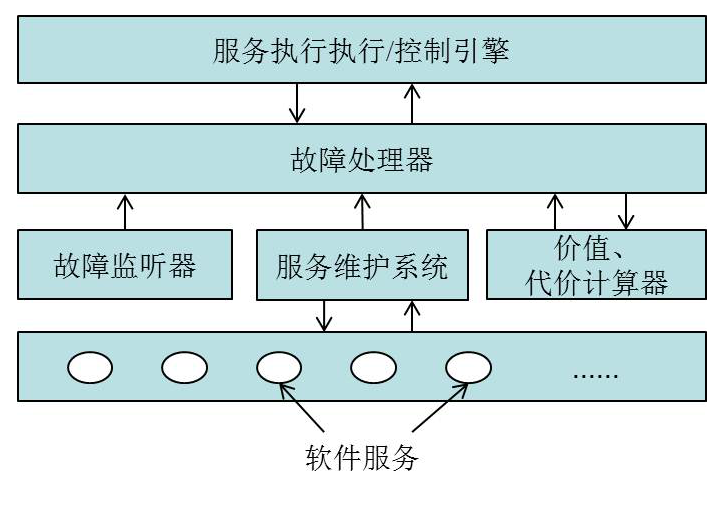
\includegraphics[width = 0.5\textwidth]{prototype_system}
    \caption{支持不确定性决策的服务原型系统结构}\label{figure:prototype_system}
    \vspace{-1em}
\end{figure}

原型系统底层由大量虚拟的~Web Service~提供支持,具有一个候选服务的维护系统,同时故障监听器和价值、代价计算器为故障处理器提供支持,使得能够决策出最优的动作。最上层是服务执行/控制引擎,类似于~BPEL~执行引擎,对组合软件服务的执行进行控制、决策和故障恢复。

拟采用的开发环境:Java语言,JDK 1.7; 运行环境:JRE 1.7 64bit,系统平台Microsoft Windows 7 64bit, 处理器为Intel® Core i3 CPU 3.0GHz,系统内存为4G,JVM分配512M内存。

拟进行三个实验:
实验1:同一服务方案下,执行过程中面对一组按时间先后次序发生的不确定性事件,分别采用~MDP~和贪心策略,对比决策效果。
实验2:针对同一服务方案,在服务失败赔偿参数~($fc$)~取不同值的情况下,对决策动作和相应收益的影响。
实验3:针对不同结构、不同规模的流程,针对一次决策所耗费时间的对比。

\subsubsection{不确性决策在海运物流中的应用验证}

\paragraph{服务方案}

%此处需要增加业务描述的QoS,需求等等
%
%业务层面的服务不同于如式(~\ref{equation:cs}~)所示的表示方式,其除了软件层面的QoS之外,还具备

业务层面的不确定性采用海运物流业务作为示例,其多方之间的工作流程如图~\ref{figure:bp_example}~所示。它实际上就是一个有向图,将其简化转换之后如图~\ref{figure:bp_ws_process}~所示。

\begin{figure}[htbp]
    \centering
    \includegraphics[width = 0.95\textwidth]{bp_example}
    \caption{海运物流工作流}\label{figure:bp_example}
    \vspace{-1em}
\end{figure}

\begin{figure}[htbp]
    \centering
    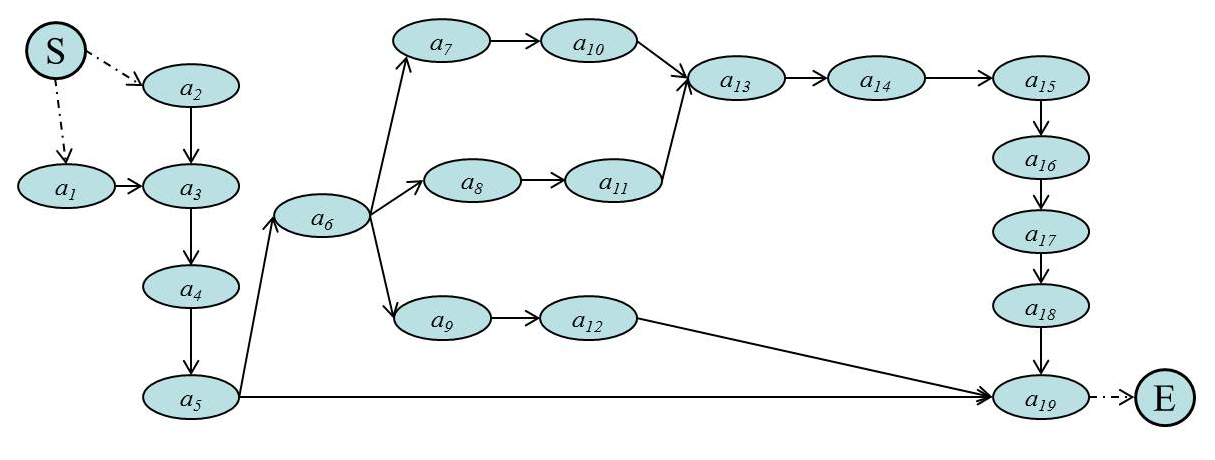
\includegraphics[width = 0.7\textwidth]{bp_ws_process}
    \caption{海运物流业务DAG图}\label{figure:bp_ws_process}
    \vspace{-1em}
\end{figure}

\paragraph{不确定性事件} \label{sec:uc_bp}

业务层面执行比软件层面有更多复杂的不确定性事件,其表示方式如式(\ref{equation:event})所示。其不确定性事件的类型除了~\ref{sec:uc_event}~节所介绍的之外,还增加两类事件:

\begin{itemize}
    
    \item 由用户产生的事件,主要指用户需求发生变化,分为以下几类:
    
    $E_{31}$:~用户所需~QoS~发生变化,包括执行时间,成本(价格),可靠性等等。
    
    $E_{32}$:~用户所需服务发生变化,主要指某个活动用户需要指定某个服务来执行,或者指定不能由某个服务来执行。
    
    $E_{33}$:~用户要求终止服务执行。
    
    \item 由服务执行方产生的事件,主要指服务执行所需的可用资源发生变化,比如海运物流中集装箱的个数由于损坏而变少,则海运无法继续按照原计划执行运输,再如航空领域由于天气原因导致的航班取消,导致于当天能够起飞的飞机数量变少(甚至于减少为0)。这两类统称为服务的可用资源发生变化,分为以下若干小类:
    
    $E_{41}$:~服务所依赖的资源减为0或者完全失效,导致于依赖于此类资源的服务完全不能执行。比如海运物流中,所承载运输的船坏了,所运输的所有物品都不能运输了。
    
    $E_{42}$:~服务所依赖的资源减少一部分,导致于服务依赖的资源不足,服务执行受到影响,但不是完全不能执行。比如海运物流中,舱位个数预留不足,导致于货物不能全部装上,此时只能寻找其他船只的舱位同时运输。
    
    
\end{itemize}

其不确定性事件在不同的活动中是不一样的,因此枚举所有活动中所有可能的不确定性事件如表~\ref{table:ocean_shipping_uc}~所示。

% Table generated by Excel2LaTeX from sheet 'Sheet8'
%\begin{table}[htbp]
%    \caption{海运物流中的不确定性}
%    \vspace{-0.5em}\label{table:ocean_shipping_uc}\centering\zihao{5}
%    \begin{tabular}{cccc}
%         \toprule
%         活动编号  & 活动描述  & 需求的不确定性 & 可用资源的不确定性 \\
%         \midrule
%         ~$a_1$~ & 发布航线信息 & -     & ~$E_{41}$~ ~$E_{42}$~ \\
%         ~$a_2$~ & 询问航线信息 & -     & ~$E_{41}$~ ~$E_{42}$~ \\
%         ~$a_3$~ & 查询、返回航线信息 & ~$E_{31}$~ ~$E_{32}$~ & ~$E_{41}$~ ~$E_{42}$~ \\
%         ~$a_4$~ & 预订舱位  & ~$E_{31}$~ ~$E_{32}$~ & - \\
%         ~$a_5$~ & 接受舱位预订 & -     & ~$E_{41}$~ ~$E_{42}$~ \\
%         ~$a_6$~ & 接受提单  & ~$E_{31}$~ ~$E_{32}$~ & ~$E_{41}$~ ~$E_{42}$~ \\
%         ~$a_7$~ & 预订集装箱 & ~$E_{31}$~ ~$E_{32}$~ & - \\
%         ~$a_8$~ & 预订卡车  & ~$E_{31}$~ ~$E_{32}$~ & - \\
%         ~$a_9$~ & 报关申请  & ~$E_{31}$~   & - \\
%         ~$a_{10}$~ & 确认集装箱预订 & -     & ~$E_{41}$~ ~$E_{42}$~ \\
%         ~$a_{11}$~ & 确认卡车预订 & -     & ~$E_{41}$~ ~$E_{42}$~ \\
%         ~$a_{12}$~ & 报关检查  & -     & ~$E_{41}$~ \\
%         ~$a_{13}$~ & 运输空箱  & ~$E_{31}$~ ~$E_{32}$~ & ~$E_{41}$~ ~$E_{42}$~ \\
%         ~$a_{14}$~ & 装载货物进集装箱 & -     & ~$E_{41}$~ ~$E_{42}$~ \\
%         ~$a_{15}$~ & 铅封集装箱 & ~$E_{32}$~   & ~$E_{41}$~ \\
%         ~$a_{16}$~ & 运输重箱  & -     & ~$E_{41}$~ ~$E_{42}$~ \\
%         ~$a_{17}$~ & 堆存货物  & ~$E_{31}$~ ~$E_{32}$~ & ~$E_{41}$~ ~$E_{42}$~ \\
%         ~$a_{18}$~ & 货物装船  & ~$E_{31}$~ ~$E_{32}$~ & ~$E_{41}$~ ~$E_{42}$~ \\
%         ~$a_{19}$~ & 运输货物至目的地 & -     & ~$E_{41}$~ \\
%         \bottomrule
%    \end{tabular}%
%\end{table}%

\begin{table}[htbp]
    \caption{海运物流中的不确定性}
    \vspace{-0.5em}\label{table:ocean_shipping_uc}\centering\zihao{5}
    \begin{tabularx}{\textwidth}{cX}
        \toprule
        活动编号  & \multicolumn{1}{c}{可能的不确定性} \\
        \midrule
        ~$a_1$~ & ~$E_{41}$:(天气原因)轮船不能航行;~$E_{42}$:(轮船损坏)轮船数量减少; \\
        ~$a_2$~ & ~$E_{41}$:(天气原因)轮船不能航行;~$E_{42}$:(轮船损坏)轮船数量减少; \\
        ~$a_3$~ & ~$E_{31}$:需求的价格/运输时间/可靠性发生变化;~$E_{32}$:用户指定需要某(种)条船;~$E_{41}$:轮船不能航行;~$E_{42}$:轮船数量减少; \\
        ~$a_4$~ & ~$E_{31}$:需求的价格发生变化;~$E_{32}$:用户指定需要某个(种)舱位; \\
        ~$a_5$~ & ~$E_{41}$:(海关原因)舱位完全不能满足;~$E_{42}$:(轮船损坏)能提供的舱位数量不足; \\
        ~$a_6$~ & ~$E_{31}$:需求的价格发生变化;~$E_{32}$:用户指定需要某个/种舱位;~$E_{41}$:舱位完全不能满足;~$E_{42}$:能提供的舱位数量不足; \\
        ~$a_7$~ & ~$E_{31}$:需求的集装箱成本变化;~$E_{32}$:用户指定更换为某批/种集装箱; \\
        ~$a_8$~ & ~$E_{31}$:需求的卡车运输成本/运输时间发生变化;~$E_{32}$:用户指定要求另一批/类型卡车运输; \\
        ~$a_9$~ & ~$E_{31}$:需求报关时间变化; \\
        ~$a_{10}$~ & ~$E_{41}$:集装箱完全不能满足;~$E_{42}$:集装箱只能满足部分需求; \\
        ~$a_{11}$~ & ~$E_{41}$:卡车完全不能满足;~$E_{42}$:卡车只能满足部分需求; \\
        ~$a_{12}$~ & ~$E_{41}$:报关被拒,完全失败; \\
        ~$a_{13}$~ & ~$E_{31}$:需求的集装箱成本变化;~$E_{32}$:用户指定更换为某批/种集装箱;~$E_{41}$:运输过程中车祸集装箱全部损坏;~$E_{42}$:运输过程中集装箱部分损坏; \\
        ~$a_{14}$~ & ~$E_{41}$:货物不能装在此类集装箱;~$E_{42}$:货物只能装部分集装箱; \\
        ~$a_{15}$~ & ~$E_{32}$:需求更换为某批/种集装箱;~$E_{41}$:车队技术工人无法上班,不能铅封; \\
        ~$a_{16}$~ & ~$E_{41}$:车队无法运输所有集装箱;~$E_{42}$:车祸损坏了部分集装箱; \\
        ~$a_{17}$~ & ~$E_{31}$:需求成本/可靠性变化;~$E_{32}$:需求更换场站;~$E_{41}$:场站不能堆存货物;~$E_{42}$:场站只能堆存部分货物; \\
        ~$a_{18}$~ & ~$E_{31}$:需求成本变化;~$E_{32}$:需求更换船只;~$E_{41}$:货物不能装船;~$E_{42}$:货物只能部分装船; \\
        ~$a_{19}$~ & ~$E_{41}$:货物中途出现问题,被退回来或不能到达; \\
        \bottomrule
    \end{tabularx}%
\end{table}%

\paragraph{服务执行的状态}

(1)~单个活动的状态
服务执行的状态仍然如~\ref{sec:service_state}~节介绍,单个活动之间的状态转换关系如图~\ref{figure:state_trans_pb}~所示。

\begin{figure}[htbp]
    \centering
    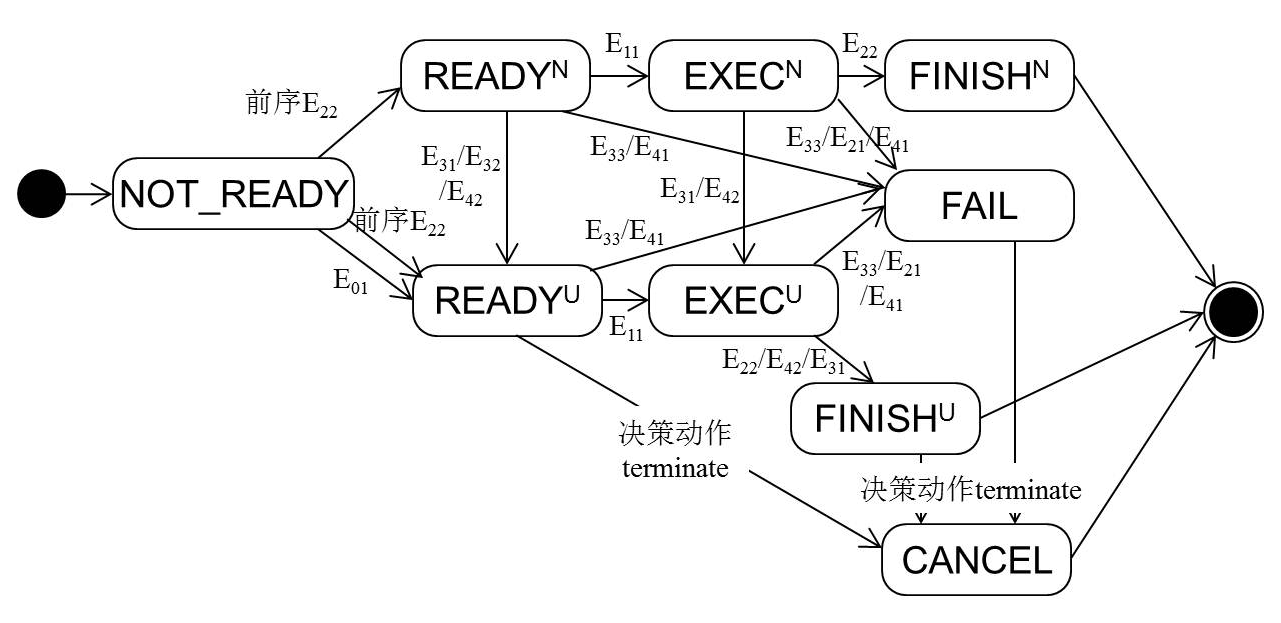
\includegraphics[width = 0.6\textwidth]{state_trans_bp}
    \caption{业务层面服务活动的状态转换关系}\label{figure:state_trans_pb}
    \vspace{-1em}
\end{figure}

业务层面服务活动之间的状态转换不同于如图~\ref{figure:state_trans}~所示的~Web Service~服务活动之间的状态转换,其不同点主要有:

1)~业务层面的不确定性事件包含了~Web Service~层面的所有不确定性事件,并具备~\ref{sec:uc_bp}~节所介绍的业务层面不确定性;

2)~业务层面在$READY$状态时会有用户的需求或者外部环境的变化,使得服务执行到另外的状态;而在纯的~Web Service~层面无需对$READY$状态的不确定性进行考虑;

3)~业务层面在$EXEC$状态也会有用户的需求或者外部环境的变化而导致于服务执行状态发生变化,甚至于引起服务执行失败;而在~Web Service~层面仅仅需要等到服务执行完的事件触发~$E_{21}/E_{22}$~。

(2)~服务执行的整体状态

在业务层面,由于不同的事件会使得流程执行到不同的状态,并且业务层面的需求和外部环境是可观察的,这与~Web Service~层面不同。因此,处理服务不确定性时需要确定是由用户需求导致的还是由外部环境变化导致的,从而整体服务流程的状态可由前锋线上的状态和不确定性事件源组合而成,如式(\ref{equation:state_total_bp})所示。

\begin{equation}\label{equation:state_total_bp}
state = < state(a_i),state(a_{i+1}),..., state(a_j), event >
\end{equation}
\begin{tabularx}{\textwidth}{@{}l@{\quad}l@{\pozhehao }X@{}}
    式中
    & $state(a_i)$ & 活动~$a_i$~的状态;\\
    & $event$ & 使得服务处于当前状态的不确定性事件,如式(\ref{equation:event})所示。
\end{tabularx}\vspace{\wordsep}

业务层面的不确定性事件也包含软件层面的不确定性事件,而软件层面的不确定性事件是不可观测的,因此若服务状态是由软件层面的不确定性事件触发,则式(\ref{equation:state_total_bp})中的~$event$~取值为~$NULL$~,此时,按照软件层面的不确定性进行决策,如表~\ref{table:state_action}~所示。

\paragraph{决策动作}

业务层面的决策动作如同软件层面的决策动作,只是决策时刻不只是在服务执行结束时,而且在服务未执行时若有不确定性事件发生也会进行决策,换句话说,决策不仅包括对当前所执行服务的决策,并对预测的非正常服务也执行决策。

同时,业务层面的不确定性一旦发生,就必须做出决策,这是因为无论用户需求发生变化还是外部环境发生变化,若不进行动作(不作为)则会导致业务执行下来不满足用户需求或者彻底失败,而这两种结果不是想要的结果。

\paragraph{事件、决策和状态之间的关系}

要对业务层面的不确定性进行决策,需要知道业务层面导致于此类不确定性的原因(事件源),即是在如图~\ref{figure:state_trans_pb}~中体现出来即指向某状态的边上的事件,于是可以根据类似表~\ref{table:state_action}~中所示的软件层面不确定性而得出业务层面不确定性,如表~\ref{table:state_action_bp}~所示,此表与如图~\ref{figure:state_trans_pb}~中的事件和状态相一致。

\begin{table}[htbp]
    \caption{服务状态与决策动作之间的关系(业务层面)}
    \vspace{-0.5em}\label{table:state_action_bp}\centering\zihao{5}
    \begin{threeparttable}
        \begin{tabular}{clclccc}
            \toprule
            事件源 & 状态类型\tnote{1} & 决策动作 & 决策后可能状态\tnote{1} & $r$~\tnote{2} & {$\Delta T$} & {$\Delta C$} \\
            \midrule
            
            %------------------------------------------------------
            {$E_{31}$} 
            & {${READY^U}$}
            & {终止}
            & {$STOP$} 
            & {0} 
            & {0} 
            & {$fc$} \\
            
            {}
            & {}
            & {替换} 
            & {$FINISH$} 
            & $R_{ik}\tnote{3}$ 
            & {\multirow{2}{*}{$T_{ik}-T_{i0}$}} 
            & {\multirow{2}{*}{$C_{ik}-C_{i0}$}} \\
            
            {}
            & {}
            & {} 
            & {$FAIL$} 
            & {0}
            & {} 
            & {} \\
            
            {}
            & {}
            & {重组} 
            & {$FINISH^{N/U}$} 
            & $R_{ik}\tnote{3}$ 
            & {\multirow{2}{*}{$\sum\limits_{x = i}^j {({T_{xk}} - {T_{x0}})} $}}
            & {\multirow{2}{*}{$\sum\limits_{x = i}^j {({C_{xk}} - {C_{x0}})} $}} \\
            
            
            {}
            & {}
            & {} 
            & {$FAIL$} 
            & {0}
            & {} 
            & {} \\
            
            %------------------------------------------------------
            {} 
            & {${FAIL}$}
            & {终止}
            & {$STOP$} 
            & {0} 
            & {0} 
            & {$fc$} \\
            
            {}
            & \multicolumn{1}{r}{$/EXEC^U$}
            & {替换} 
            & {${FINISH}^{N/U}$} 
            & $R_{ik}\tnote{3}$ 
            & {\multirow{2}{*}{$T_{ik}$}} 
            & {\multirow{2}{*}{$C_{ik}$}} \\
            
            {}
            & {}
            & {} 
            & {$FAIL$} 
            & {0}
            & {} 
            & {} \\
            
            {}
            & {}
            & {重组} 
            & {$FINISH^{N/U}$} 
            & $R_{ik}\tnote{3}$ 
            & {\multirow{2}{*}{$T_{i0}+\sum\limits_{x = i}^j {({T_{xk}} - {T_{x0}})} $}}
            & {\multirow{2}{*}{$C_{i0}+\sum\limits_{x = i}^j {({C_{xk}} - {C_{x0}})} $}} \\
            
            
            {}
            & {}
            & {} 
            & {$FAIL$} 
            & {0}
            & {} 
            & {} \\
            
            %------------------------------------------------------
            {} 
            & {${FINISH^U}$}
            & {终止}
            & {$STOP$} 
            & {0} 
            & {0} 
            & {$fc$} \\
            
            {}
            & {}
            & {重组} 
            & {$FINISH^{N/U}$} 
            & $R_{ik}\tnote{3}$ 
            & {\multirow{2}{*}{$\sum\limits_{x = i}^j {({T_{xk}} - {T_{x0}})} $}}
            & {\multirow{2}{*}{$\sum\limits_{x = i}^j {({C_{xk}} - {C_{x0}})} $}} \\
            
            
            {}
            & {}
            & {} 
            & {$FAIL$} 
            & {0}
            & {} 
            & {} \\
            %------------------------------------------------------
            {$E_{32}$} 
            & {$READY^U$}
            & {替换} 
            & {$FINISH$} 
            & $R_{ik}\tnote{3}$ 
            & {\multirow{2}{*}{$T_{ik}-T_{i0}$}} 
            & {\multirow{2}{*}{$C_{ik}-C_{i0}$}} \\
            
            {}
            & {}
            & {} 
            & {$FAIL$} 
            & {0}
            & {} 
            & {} \\
            
            {}
            & {}
            & {重组} 
            & {$FINISH^{N/U}$} 
            & $R_{ik}\tnote{3}$ 
            & {\multirow{2}{*}{$\sum\limits_{x = i}^j {({T_{xk}} - {T_{x0}})} $}}
            & {\multirow{2}{*}{$\sum\limits_{x = i}^j {({C_{xk}} - {C_{x0}})} $}} \\
            
            
            {}
            & {}
            & {} 
            & {$FAIL$} 
            & {0}
            & {} 
            & {} \\
            
            %------------------------------------------------------
            {$E_{33}$} 
            & {${READY^U}$}
            & {终止}
            & {$STOP$} 
            & {0} 
            & {0} 
            & {$fc$} \\
            %------------------------------------------------------
            {$E_{41}$} 
            & {${FAIL^U}$}
            & {终止}
            & {$STOP$} 
            & {0} 
            & {0} 
            & {$fc$} \\
            
            {}
            & {}
            & {替换} 
            & {$FINISH$} 
            & $R_{ik}\tnote{3}$ 
            & {\multirow{2}{*}{$T_{ik}$}} 
            & {\multirow{2}{*}{$C_{ik}$}} \\
            
            {}
            & {}
            & {} 
            & {$FAIL$} 
            & {0}
            & {} 
            & {} \\
            
            {}
            & {}
            & {重组} 
            & {$FINISH^{N/U}$} 
            & $R_{ik}\tnote{3}$ 
            & {\multirow{2}{*}{$T_{i0}+\sum\limits_{x = i}^j {({T_{xk}} - {T_{x0}})} $}}
            & {\multirow{2}{*}{$C_{i0}+\sum\limits_{x = i}^j {({C_{xk}} - {C_{x0}})} $}} \\
            
            
            {}
            & {}
            & {} 
            & {$FAIL$} 
            & {0}
            & {} 
            & {} \\
            %------------------------------------------------------
            {$E_{42}$} 
            & {${READY^U}$}
            & {终止}
            & {$STOP$} 
            & {0} 
            & {0} 
            & {$fc$} \\
            
            {}
            & {}
            & {替换} 
            & {$FINISH$} 
            & $R_{ik}\tnote{3}$ 
            & {\multirow{2}{*}{$T_{ik}-T_{i0}$}} 
            & {\multirow{2}{*}{$C_{ik}-C_{i0}$}} \\
            
            {}
            & {}
            & {} 
            & {$FAIL$} 
            & {0}
            & {} 
            & {} \\
            
            {}
            & {}
            & {重组} 
            & {$FINISH^{N/U}$} 
            & $R_{ik}\tnote{3}$ 
            & {\multirow{2}{*}{$\sum\limits_{x = i}^j {({T_{xk}} - {T_{x0}})} $}}
            & {\multirow{2}{*}{$\sum\limits_{x = i}^j {({C_{xk}} - {C_{x0}})} $}} \\
            
            
            {}
            & {}
            & {} 
            & {$FAIL$} 
            & {0}
            & {} 
            & {} \\
            %------------------------------------------------------
            {} 
            & {${EXEC^U}$}
            & {终止}
            & {$STOP$} 
            & {0} 
            & {0} 
            & {$fc$} \\
            
            {}
            & \multicolumn{1}{r}{$/FINISH^U$}
            & {替换} 
            & {$FINISH$} 
            & $R_{ik}\tnote{3}$ 
            & {\multirow{2}{*}{$T_{ik}$}} 
            & {\multirow{2}{*}{$C_{ik}$}} \\
            
            {}
            & {}
            & {} 
            & {$FAIL$} 
            & {0}
            & {} 
            & {} \\
            
            {}
            & {}
            & {重组} 
            & {$FINISH^{N/U}$} 
            & $R_{ik}\tnote{3}$ 
            & {\multirow{2}{*}{$T_{i0}+\sum\limits_{x = i}^j {({T_{xk}} - {T_{x0}})} $}}
            & {\multirow{2}{*}{$C_{i0}+\sum\limits_{x = i}^j {({C_{xk}} - {C_{x0}})} $}} \\
            
            
            {}
            & {}
            & {} 
            & {$FAIL$} 
            & {0}
            & {} 
            & {} \\
            
            \bottomrule
        \end{tabular}%
        
        \begin{tablenotes}
            \item[1] 决策动作前状态所带参数为$(T,C)$, 决策后状态参数变为~$(T+\Delta T, C+\Delta C)$,~ 其中~$\Delta T \ge 0$, ~$\Delta C \ge 0$~; 
            \item[2] $r$~为决策后,服务可继续执行的概率;
            \item[3] $S_{ik}$~为替换后的服务或者重组后最先执行的服务,~$R_{ik}$~为此服务的可靠性。
        \end{tablenotes}
    \end{threeparttable}
\end{table}%

\paragraph{决策收益}

决策收益的计算方式与~\ref{sec:reward_section}~节介绍的软件层面的决策收益一致,其中~$r$~、~$\Delta T$~、 ~$\Delta C$~的计算方式如表~\ref{table:state_action_bp}~右侧的三列所示。

\paragraph{不确定性触发关系图}

业务层面不确定性触发关系图同~\ref{sec:utg}~介绍一样。

\paragraph{海运物流业务的不确定性决策系统}

在海运物流中,如图~\ref{figure:bp_example}~所示的业务流程,可针对每个可~IT~化的活动,开发出支持此活动的~Web Service~(例如图~\ref{figure:bp_example}~所示的活动~$a_{4}$~:预订舱位),而其余只能人工作的活动(例如图~\ref{figure:bp_example}~所示的活动~$a_{14}$~:装箱)则无需开发。

开发软件层面的原型系统之后,针对海运物流的具体业务流程,开发针对海运物流的不确定性决策系统,其底层由软件层面的原型系统提供支持,上层运行海运物流的业务流程。其系统结构如图~\ref{figure:app_system}~所示。

\begin{figure}[htbp]
    \centering
    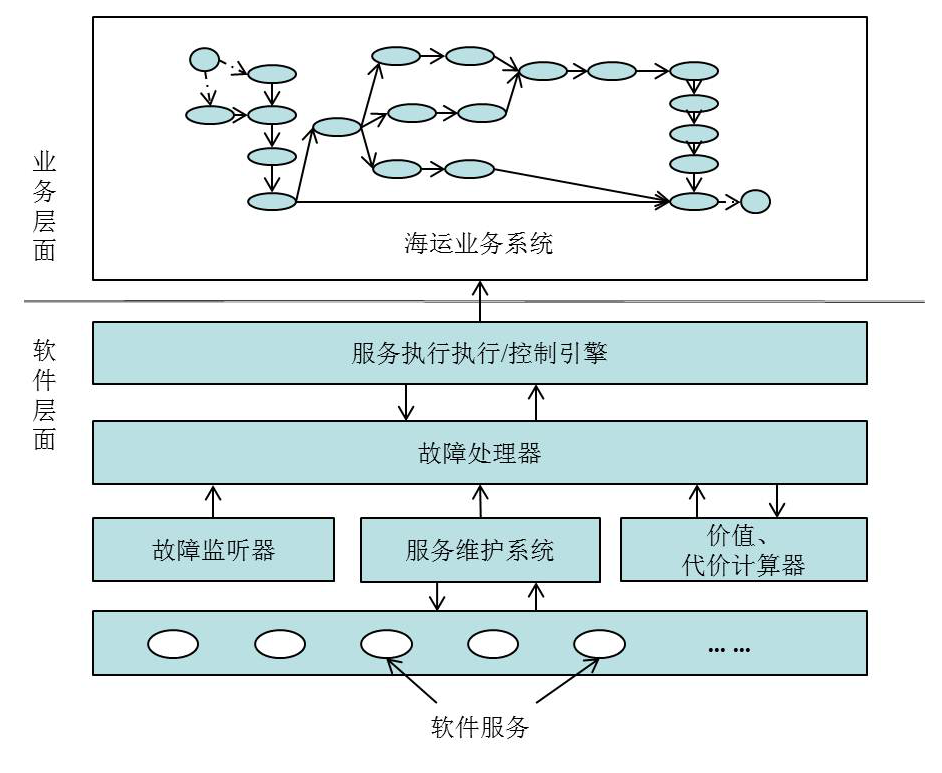
\includegraphics[width = 0.7\textwidth]{app_system}
    \caption{支持不确定性决策的海运物流业务系统结构}\label{figure:app_system}
    \vspace{-1em}
\end{figure}

%-------------------------------------------

\subsection{预期达到的目标和取得的研究成果}

对不确定性建模进行完整细化并开发出原型系统进行仿真,通过与传统的不决策或者贪心决策方式对比,从而证明本课题的研究价值。并且,开发一个针对海运物流的应用系统,其中嵌入本课题的不确定性决策的原型系统作为中间件,从而实现海运物流的不确定性决策的自动化,进一步证明本课题具有很强的研究价值。

\subsection{进度安排}
\begin{itemize}
    \item 2012/09/15-2012/10/15~完成不确定性软件层面建模(理论研究)
    \item 2012/10/15-2012/12/01~完成不确定性业务层面建模(海运业务分析)
    \item 2012/12/01-2013/01/01~完成不确定性原型系统架构设计
    \item 2013/01/01-2013/02/15~开发和测试软件层面的原型系统
    \item 2013/02/15-2013/05/01~开发和测试业务层面的应用系统
    \item 2013/05/01-2013/06/10~撰写论文
    \item 2013/06/10-2013/06/20~准备答辩
\end{itemize}




%% !Mode:: "TeX:UTF-8" 
\section{标题1}
\subsection{标题1.1}
文本1文本1文本1文本1文本1文本1文本1文本1文本1文本1文本1文本1文本1文本1文本1文本1文本1文本1文本1文本1文本1文本1文本1文本1文本1文本1文本1文本1文本1文本1文本1文本1文本1文本1文本1~http://www.imagemagick.org/script/command-line-options.php\#resize~。
%\vspace{-1.62em}

文本2文本2文本2文本2文本2文本2文本2文本2文本2文本2文本2文本2文本2文本2文本2文本2文本2文本2文本2文本2文本2文本2文本2文本2文本2文本2文本2文本2文本2文本2文本2文本2文本2文本2文本2文本2

文本3文本3文本3文本3文本3文本3文本3文本3文本3文本3文本3文本3文本3文本3文本3文本3文本3文本3文本3文本3文本3文本3文本3文本3文本3文本3文本3文本3文本3文本3文本3文本3文本3文本3文本3文本3

\subsection{标题1.2}
文本1文本1文本1文本1文本1文本1文本1文本1文本1文本1文本1文本1文本1文本1文本1文本1文本1文本1文本1文本1文本1文本1文本1文本1文本1文本1文本1文本1文本1文本1文本1文本1文本1文本1文本1

文本2文本2文本2文本2文本2文本2文本2文本2文本2文本2文本2文本2文本2文本2文本2文本2文本2文本2文本2文本2文本2文本2文本2文本2文本2文本2文本2文本2文本2文本2文本2文本2文本2文本2文本2文本2

文本3文本3文本3文本3文本3文本3文本3文本3文本3文本3文本3文本3文本3文本3文本3文本3文本3文本3文本3文本3文本3文本3文本3文本3文本3文本3文本3文本3文本3文本3文本3文本3文本3文本3文本3文本3

\subsection{标题1.3}

文本1文本1文本1文本1文本1文本1文本1文本1文本1文本1文本1文本1文本1文本1文本1文本1文本1文本1文本1文本1文本1文本1文本1文本1文本1文本1文本1文本1文本1文本1文本1文本1文本1文本1文本1

文本2文本2文本2文本2文本2文本2文本2文本2文本2文本2文本2文本2文本2文本2文本2文本2文本2文本2文本2文本2文本2文本2文本2文本2文本2文本2文本2文本2文本2文本2文本2文本2文本2文本2文本2文本2

文本3文本3文本3文本3文本3文本3文本3文本3文本3文本3文本3文本3文本3文本3文本3文本3文本3文本3文本3文本3文本3文本3文本3文本3文本3文本3文本3文本3文本3文本3文本3文本3文本3文本3文本3文本3
%% !Mode:: "TeX:UTF-8" 
\section{图片的插入方法}
\subsection{研究生院的插图规范}
图应有自明性。插图应与文字紧密配合,文图相符,内容正确。选图要力求精练,插图、照片应完整清晰。图中文字和数字等字号用宋体~5~号字。

机械工程图:采用第一角投影法,严格按照~GB4457~GB131-83《机械制图》标准规定。

数据流程图、程序流程图、系统流程图等按~GB1526-89~标准规定。

电气图:图形符号、文字符号等应符合附录~3~所列有关标准的规定。

流程图:必须采用结构化程序并正确运用流程框图。

对无规定符号的图形应采用该行业的常用画法。

坐标图的坐标线均用细实线,粗细不得超过图中曲线,有数字标注的坐标图,必须注明坐标单位。

照片图要求主题和主要显示部分的轮廓鲜明,便于制版。如用放大或缩小的复制品,必须清晰,反差适中。照片上应有表示目的物尺寸的标度。

引用文献图表必须标注出处。


\subsubsection{图题及图中说明}
每个图均应有图题(由图序和图名组成),图名在图序之后空一格排写。图序按章编排,如第~1~章第一个插图的图号为“图~1-1”等。
图题置于图下,硕士论文可只用中文书写,博士论文用中、英文两种文字居中书写,中文在上,要求中文用宋体~5~号字,英文用~Times New Roman 5~号字。有图注或其它说明时应置于图题之上。引用图应注明出处,在图题右上角加引用文献号。
图中若有分图时,分图题置于分图之下或图题之下,分图号用~a)、b)等表示。

图中各部分说明应采用中文(引用的外文图除外)或数字项号,各项文字说明置于图题之上(有分图题者,置于分图题之上)。

\subsubsection{插图编排}
插图之前,文中必须有关于本插图的提示,如“见图~1-1”、“如图~1-1~所示”等。插图与其图题为一个整体,不得拆开排写于两页。
插图处的该页空白不够排写该图整体时,则可将其后文字部分提前排写,将图移到次页。

\subsection{\LaTeX~中推荐使用的图片格式}
在~\LaTeX~中应用最多的图片格式是~EPS(Encapsulated PostScript)格式,它是一种专用的打印机描述语言,常用于印刷或打印输出。
EPS~格式图片可通过多种方式生成,这里介绍一款功能强大的免费图片处理软件------ImageMagick,
360~软件管家也提供此软件的下载。此软件可将其它格式图片转换为~EPS~格式图片,同时还可以锐化图片,使图片的局部清晰一些。

此软件对图片的格式转换操作都是在命令提示符(cmd.exe)中实现的,可以通过“开始$\to$运行$\to$输入~cmd$\to$回车”或
“开始$\to$程序$\to$附件$\to$命令提示符”找到它。在命令提示符下,首先采用“盘符命令”或“cd~命令”将当前目录改为待处理图片所在的目录,
在此目录下就可通过~convert~命令将图片转换为~EPS~格式,其命令的语法格式为

\noindent\verb|convert [可选参数] 原文件名.原扩展名 新文件名.eps|

\noindent 若~convert~命令中无可选参数,则将原来的图片格式直接转换为~EPS~格式,对图片不进行任何处理,这也是最常用的方法。
也可以选用可选参数,可选参数有很多选择,但最常用的有如下两个:

\verb|-sharpen radius{xsigma}|———此参数用来锐化图片,一般用在图片像素不高,需要提高图片清晰度的情况下。其中~radius~只能为整数,
它用来确定转换命令采取哪一种锐化算法,我们可以只取~radius~为~0;sigma~为所采取算法的锐化度,它的取值为~0.1--3~之间的任意一个浮点数,
数值越大,锐化程度也越大,通常取为~0.5--1~之间;x在参数中为分隔符。

\verb|-resize geometry|———此参数用来改变图片的大小,若图片的存储空间过大,可通过此命令缩小图片尺寸,但同时也将导致图片像素降低,
其具体用法请参见-resize geometry~的官方说明~http://www.imagemagick.org/script/command-line-options.php\#resize~

除此之外,一些文字处理软件和科学计算软件也支持生成~EPS~格式的文件,请使用“另存为”功能查看某款软件是否能够将图片以~EPS~格式的形式保存。

\subsection{单张图片的插入方法}
单张图片独自占一行的插入形式如图~\ref{golfer1}~所示。
\begin{figure}[htbp]
\centering
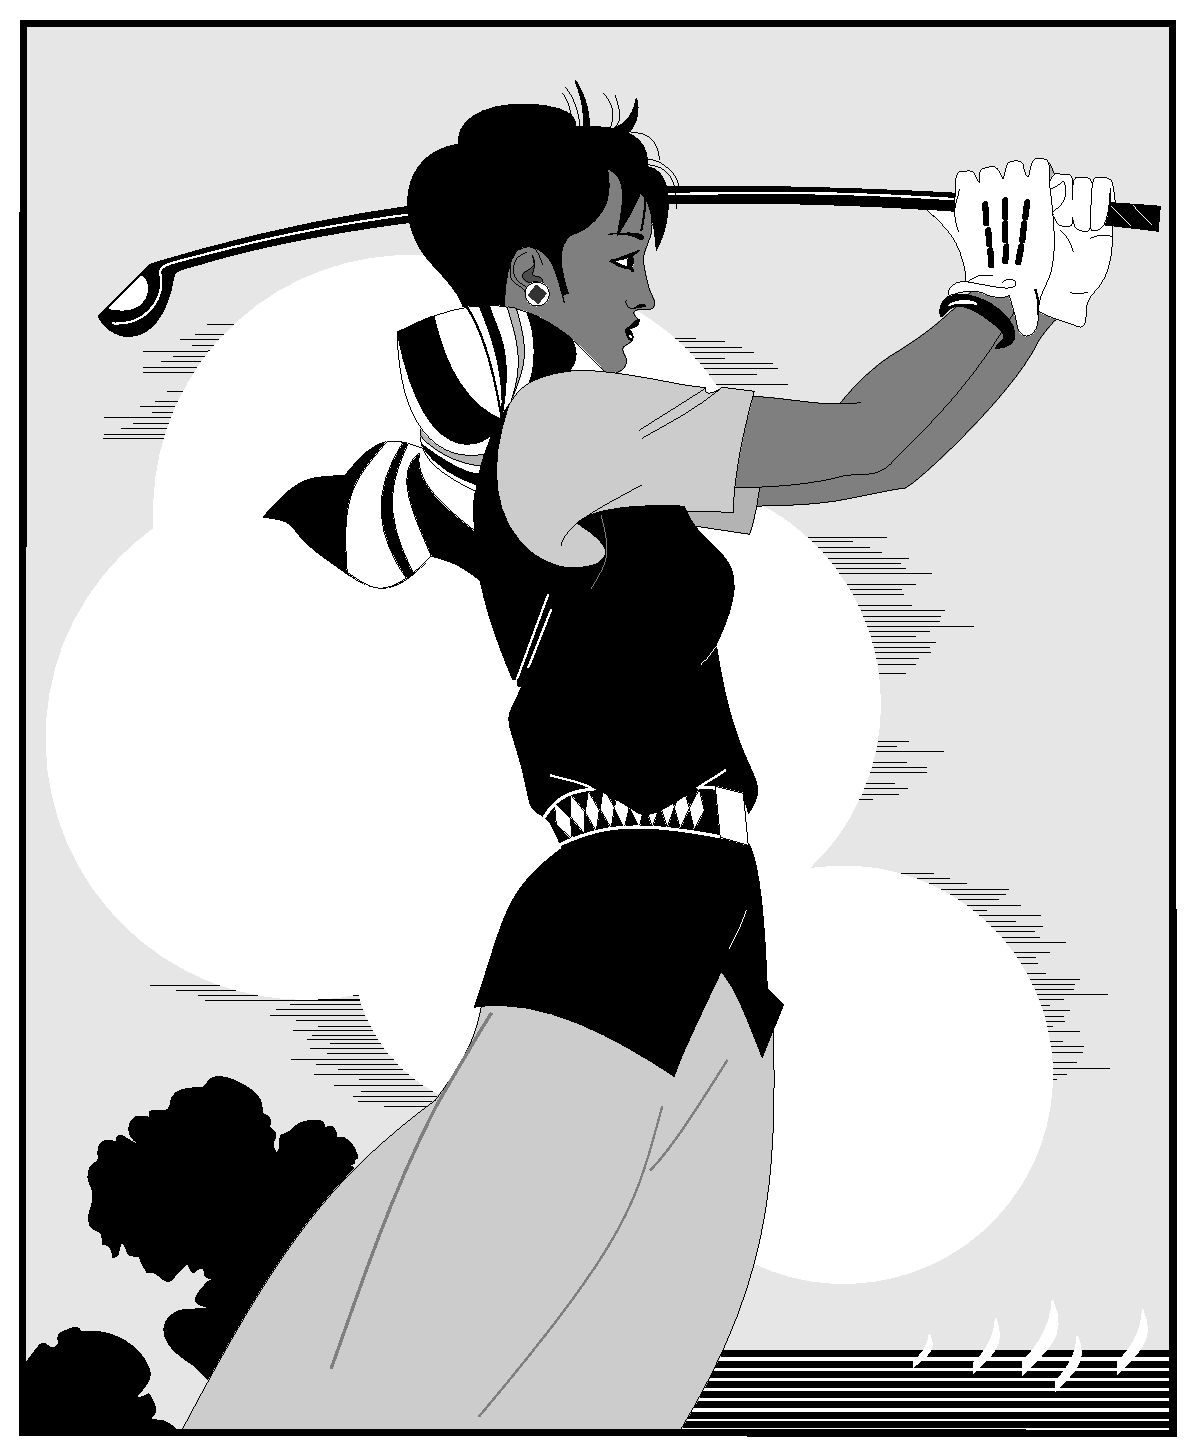
\includegraphics[width = 0.4\textwidth]{golfer}
\caption{打高尔夫球的人}\label{golfer1}
\vspace{-1em}
\end{figure}

其插入图片的代码及其说明如下。
\vspace{1em}\noindent\hrule
\begin{verbatim}
\begin{figure}[htbp]
\centering
\includegraphics[width=0.4\textwidth]{文件名(.eps)}
\caption{图片标题}\label{标签名(英文)}\vspace{-1em}
\end{figure}
\end{verbatim}
\noindent\hrule
\begin{verbatim}
figure环境的可选参数[htbp]表示浮动图形所放置的位置,h (here)表示当前位置,t (top)表示页芯顶部,b (bottom)表示页芯底部,p (page)表示单独一页。在word等软件中,图片通常插入到当前位置,如果当前页的剩余空间不够,图片将被移动到下一页,当前页就会出现很大的空白,其人工调整工作非常不便。由LaTeX提供的浮动图片功能,总是会按h->t->b->p的次序处理选项中的字母,自动调整图片的位置,大大减轻了工作量。
\centering命令将后续内容转换成每行皆居中的格式。
“\includegraphics”的可选参数用来设置图片插入文中的水平宽度,一般表示为正文宽度(\textwidth)的倍数。
\caption命令可以为图片或表格插入标题。
\label可为图片、表格或公式设置英文标签,一般不以图片或表格的数字顺序作为标签,而应包含一定的图片或表格信息,以便于文中引用(若图片、表格、公式、章节和参考文献等在文中出现的先后顺序发生了变化,其标注序号及其文中引用序号也会跟着发生变化,这一点是word等软件所不能做到的)。另外,图题或表题并不会因为分页而与图片或表格体分置于两页,章节等各级标题也不会置于某页的最底部,LaTeX系统会自动调整它们在正文中的位置,这也是word等软件所无法匹敌的。
\vspace将产生一定高度的竖直空白,必选参数为负值表示将后续文字位置向上提升,参数值可自行调整。em为长度单位,相当于大写字母M的宽度。
引用方法:“见图~\ref{标签名(英文)}”、“如图~\ref{标签名(英文)}~所示”等。
\end{verbatim}
\noindent\hrule\vspace{1em}
若需要将~2~张及以上的图片并排插入到一行中,则需要采用\verb|minipage|环境,如图~\ref{golfer2}~和图~\ref{golfer3}~所示。
\begin{figure}[htbp]
\centering
\begin{minipage}{0.4\textwidth}
\centering
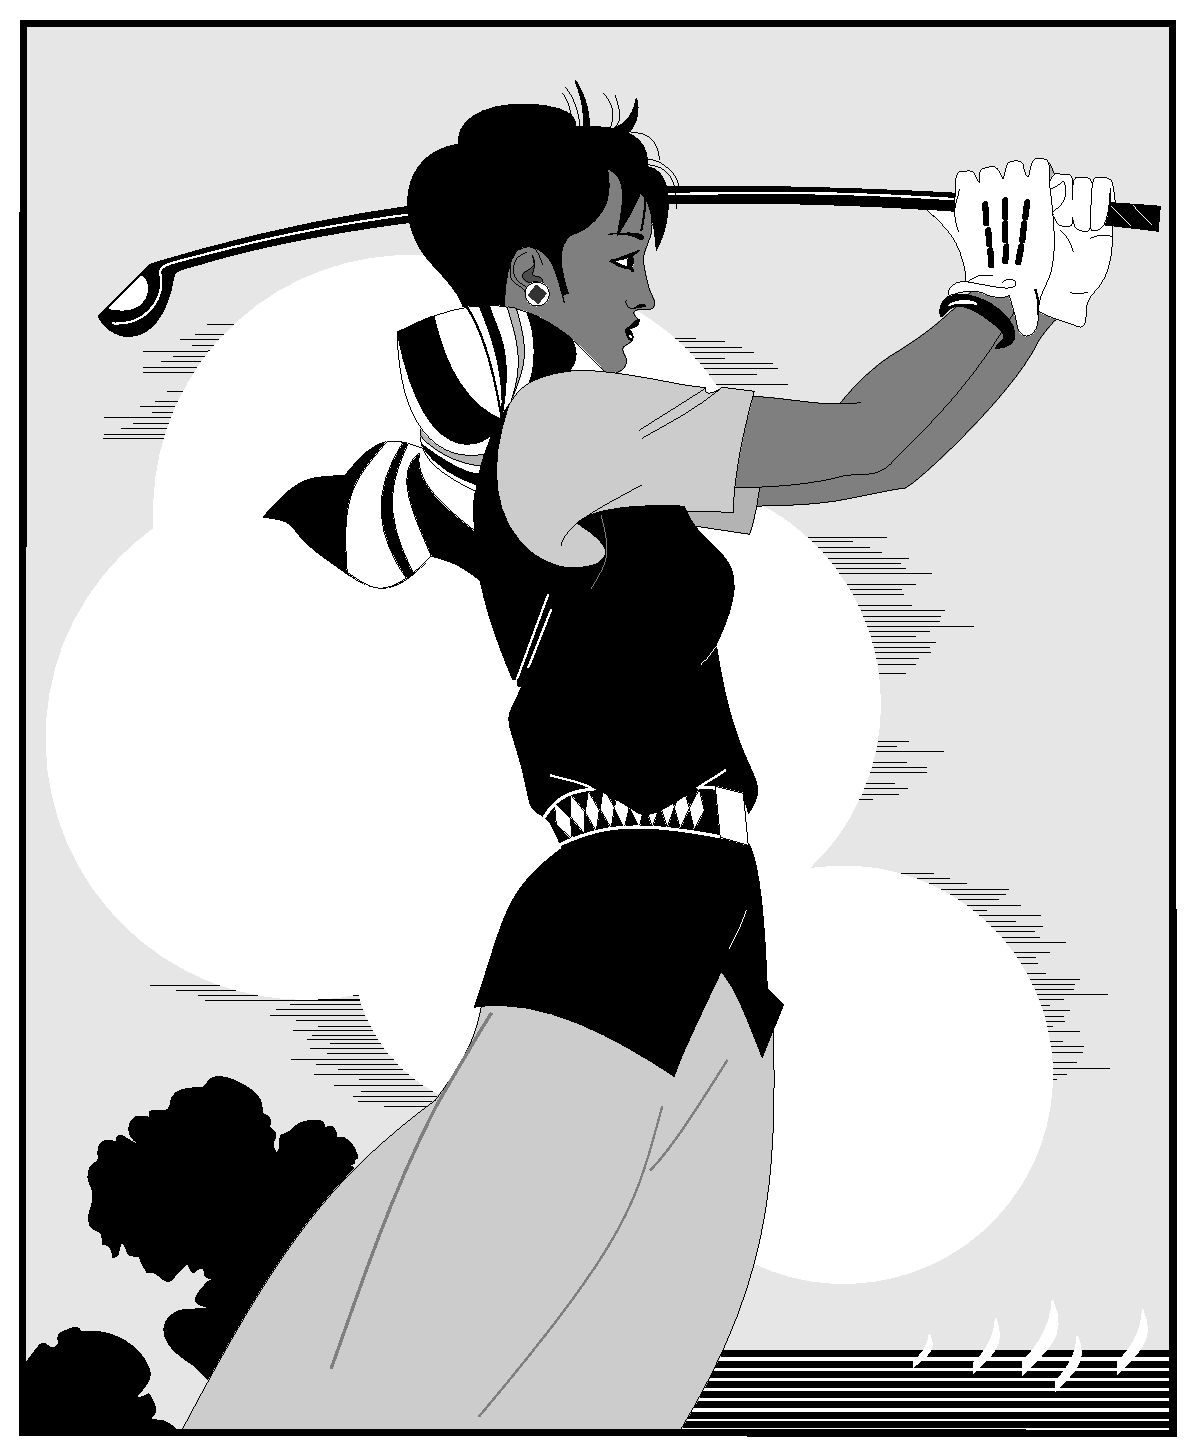
\includegraphics[width=\textwidth]{golfer}
\caption{打高尔夫球的人}\label{golfer2}
\end{minipage}
\begin{minipage}{0.4\textwidth}
\centering
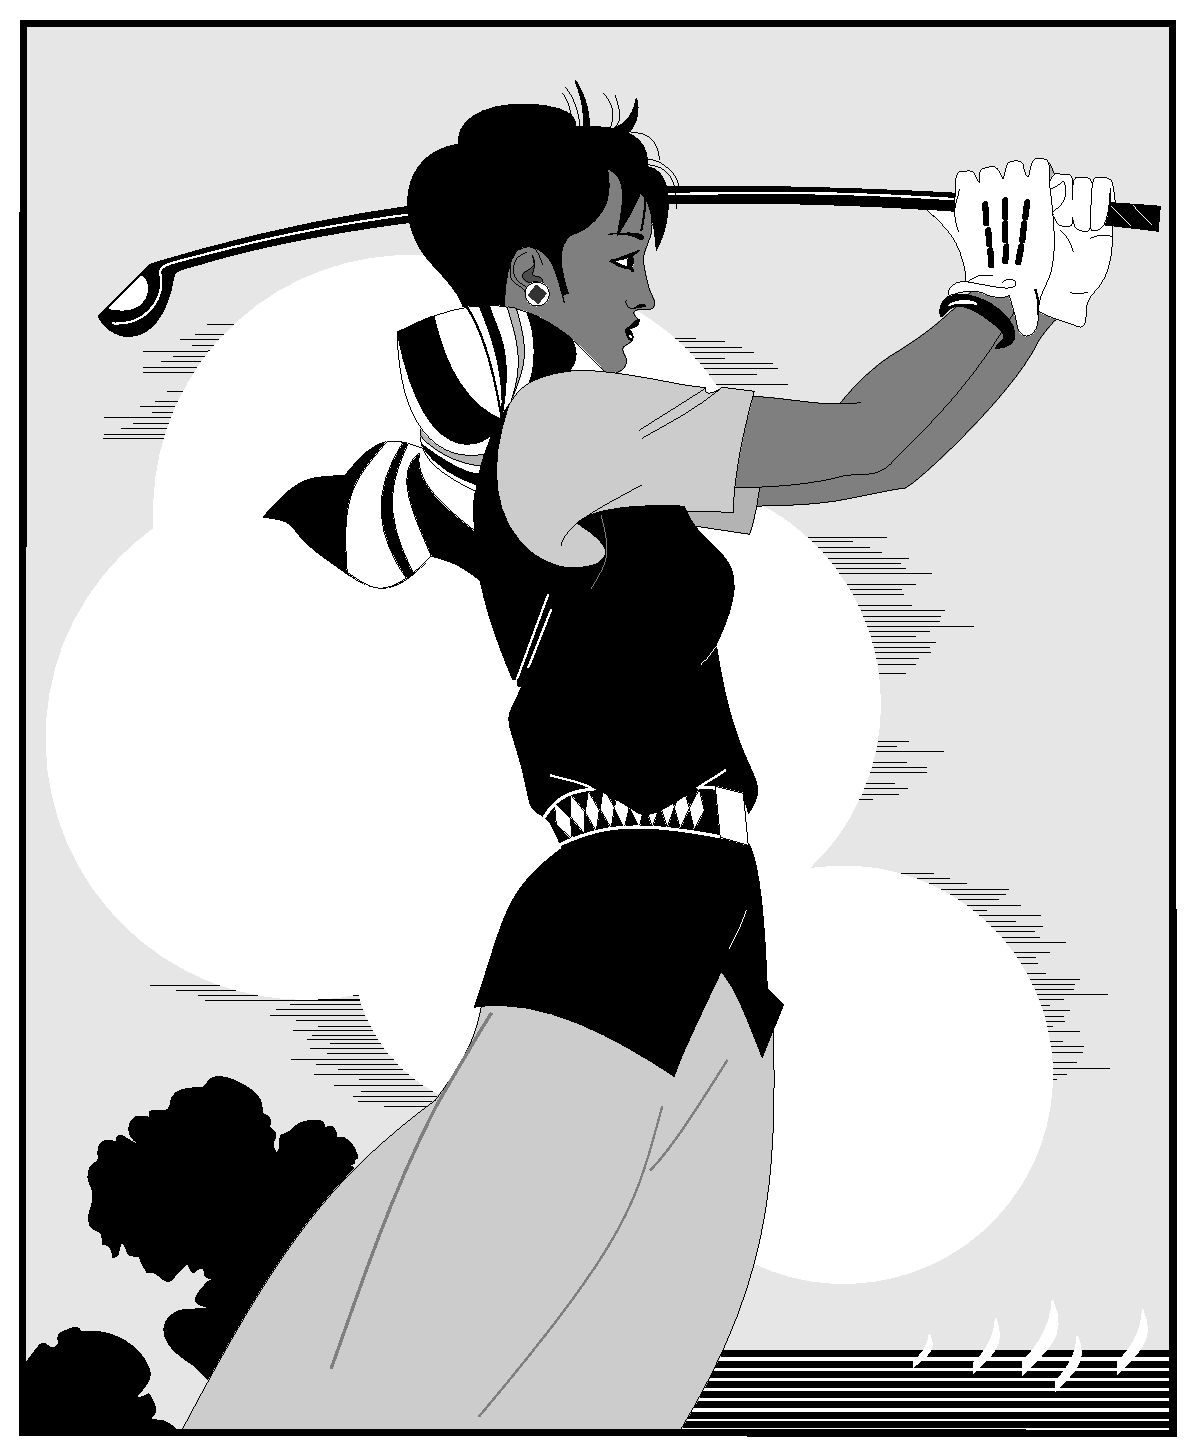
\includegraphics[width=\textwidth]{golfer}
\caption{打高尔夫球的人}\label{golfer3}
\end{minipage}\vspace{-1em}
\end{figure}

其代码如下所示。
\vspace{1em}\noindent\hrule
\begin{verbatim}
\begin{figure}[htbp]
\centering
\begin{minipage}{0.4\textwidth}
\centering
\includegraphics[width=\textwidth]{文件名}
\caption{图片标题}\label{标签名}
\end{minipage}
\begin{minipage}{0.4\textwidth}
\centering
\includegraphics[width=\textwidth]{文件名}
\caption{图片标题}\label{标签名}
\end{minipage}\vspace{-1em}
\end{figure}
\end{verbatim}
\noindent\hrule
\begin{verbatim}
minipage环境的必选参数用来设置小页的宽度,若需要在一行中插入n个等宽图片,则每个小页的宽度应略小于(1/n)\textwidth。
\end{verbatim}
\noindent\hrule

\subsection{具有子图的图片插入方法}

图中若含有子图时,需要调用~subfigure~宏包,如图~\ref{golfer4}~所示。

\begin{figure}[htbp]
\centering
\subfigure[打高尔夫球的人]{\label{golfer41}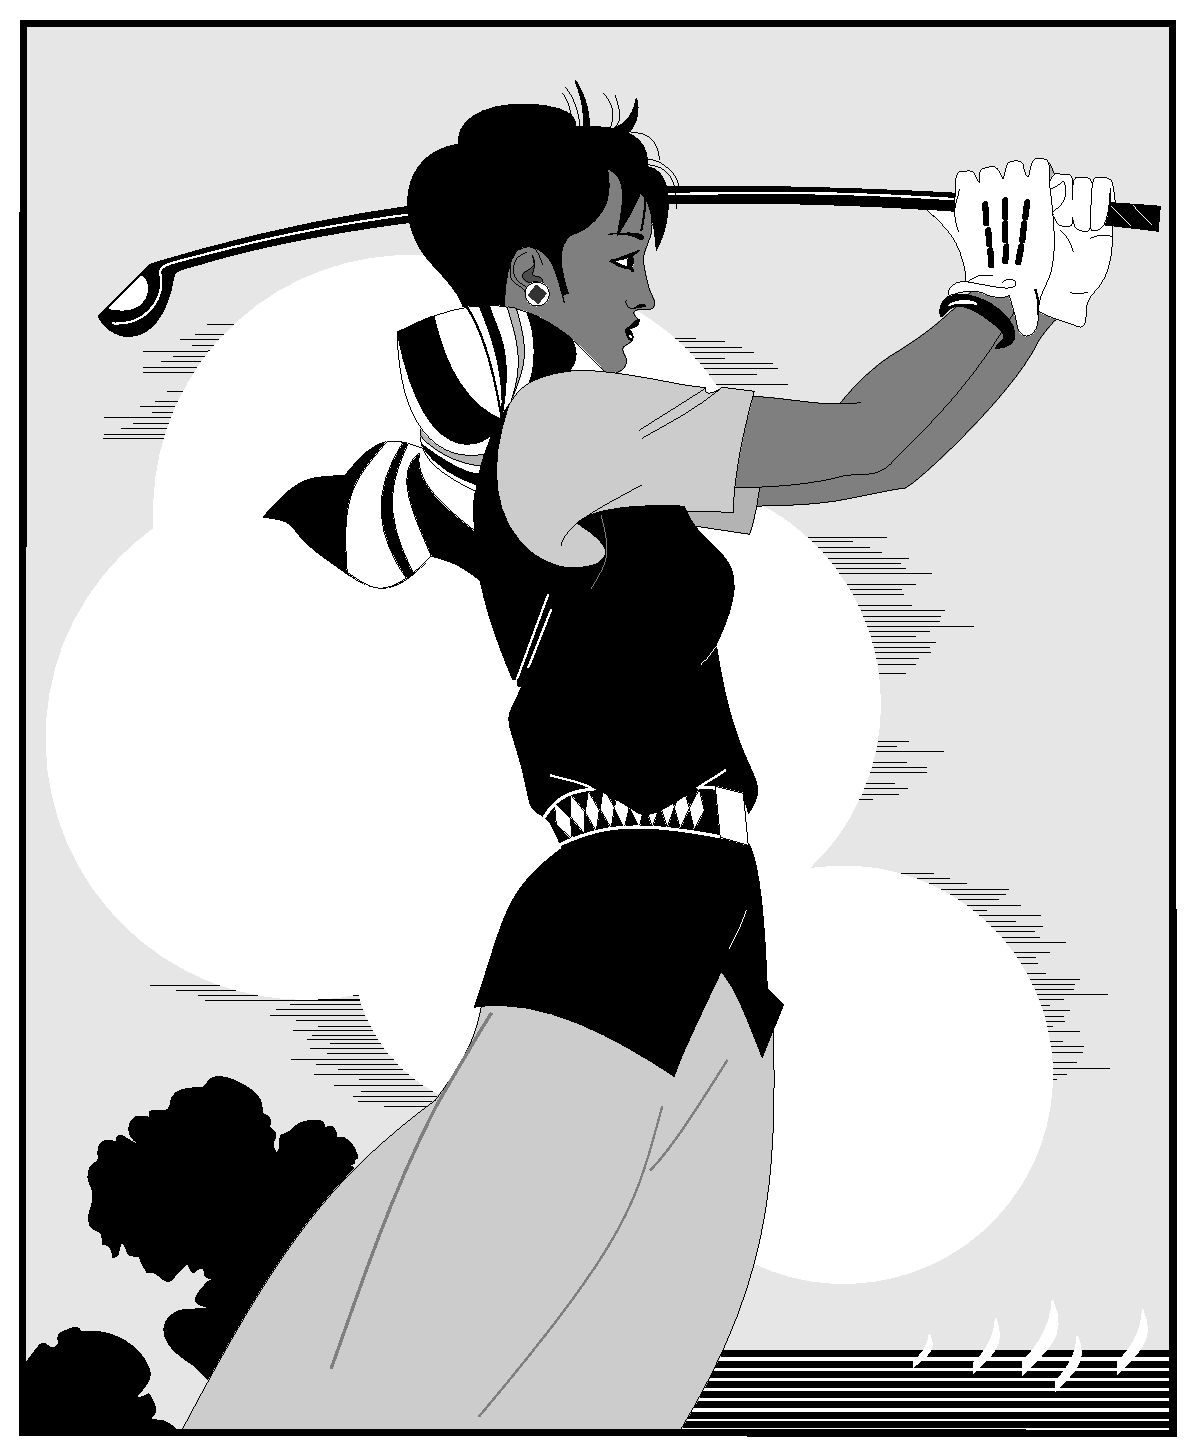
\includegraphics[width=0.4\textwidth]{golfer}}
\subfigure[打高尔夫球的人]{\label{golfer42}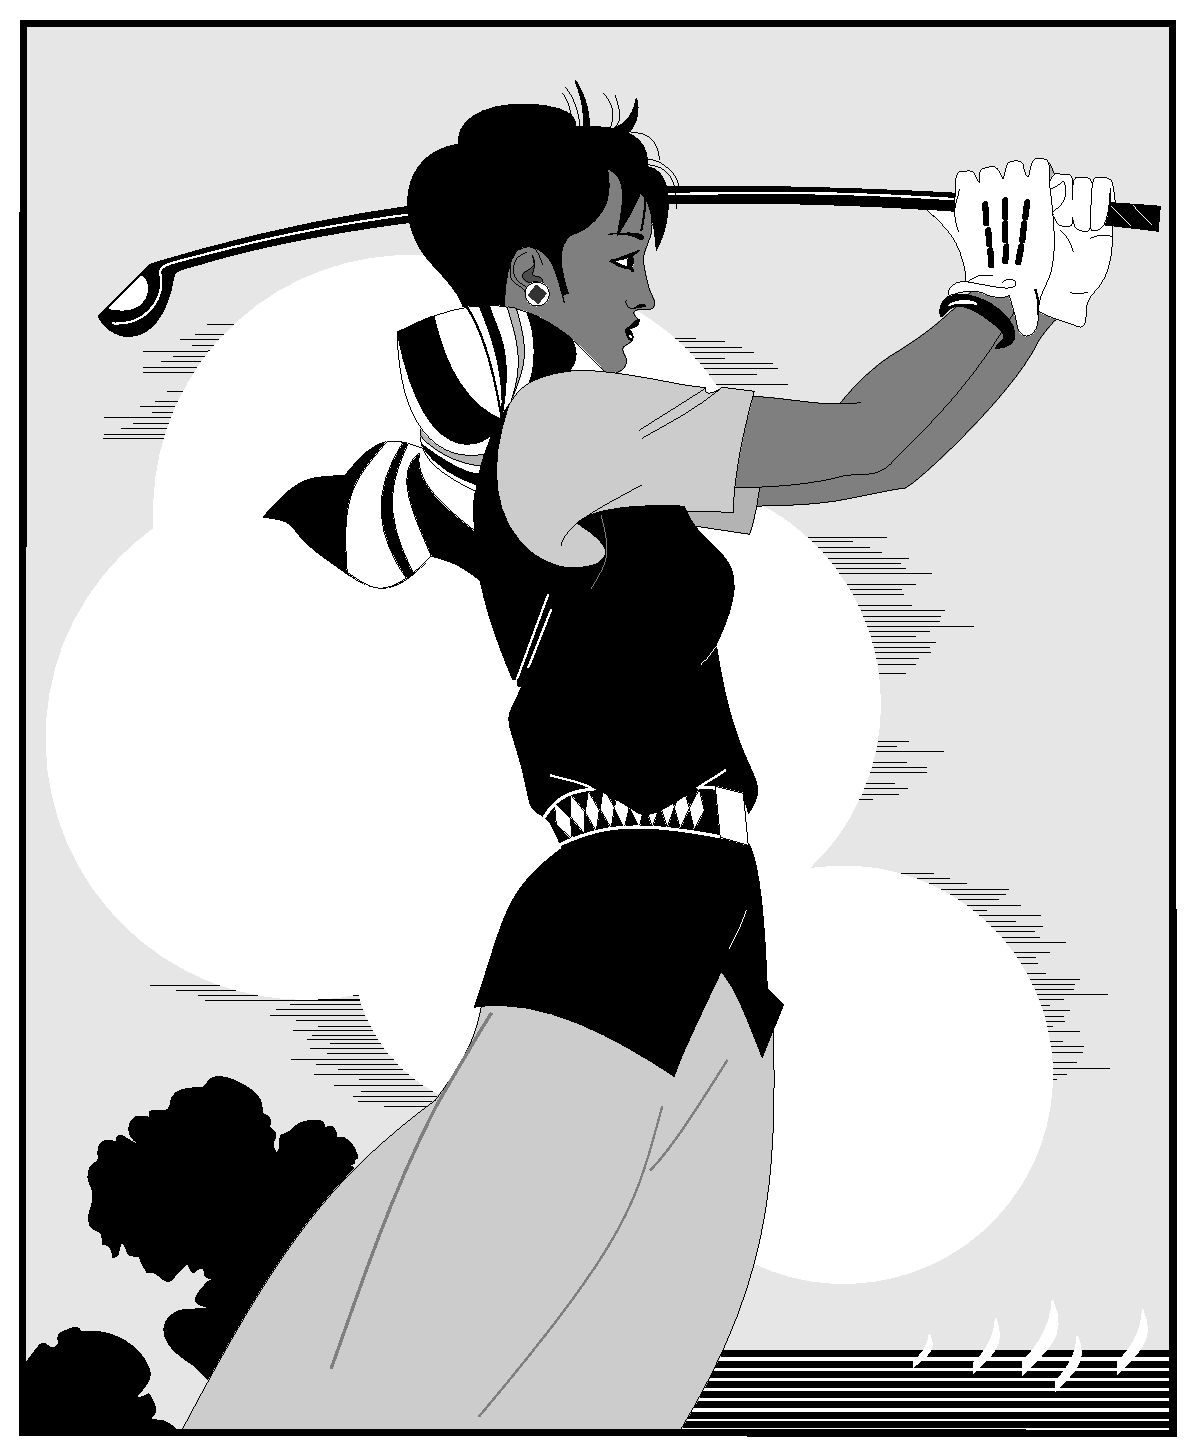
\includegraphics[width=0.4\textwidth]{golfer}}
\caption{打高尔夫球的人}\label{golfer4}\vspace{-1em}
\end{figure}

其代码及其说明如下。
\vspace{1em}\noindent\hrule
\begin{verbatim}
\begin{figure}[htbp]
\centering
\subfigure[第1个子图标题]{\label{第1个子图标签名}
                          \includegraphics[width=0.4\textwidth]{文件名}}
\subfigure[第2个子图标题]{\label{第2个子图标签名}
                          \includegraphics[width=0.4\textwidth]{文件名}}
\caption{中文总标题}\label{总标签名}
\vspace{-1em}
\end{figure}
\end{verbatim}
\noindent\hrule
\begin{verbatim}
引用方法:总图的引用方法同本章第1节,子图的引用方法用\ref{第n个子图标签名}来代替。
\end{verbatim}
\noindent\hrule\vspace{1em}

子图的引用示例:如图~\ref{golfer41}~和图~\ref{golfer42}~所示。

若想获得插图方法的更多信息,请参见网络上的~
Using Imported Graphics in \LaTeX and pdf\LaTeX~文档~http://tug.ctan.org/cgi-bin/ctanPackageInformation.py?id=epslatex。 
%% !Mode:: "TeX:UTF-8" 

\section{表格的绘制方法}
\subsection{研究生院的绘表规范}

表应有自明性。表格不加左、右边线。表的编排建议采用国际通行的三线表。表中文字用宋体~5~号字。

每个表格均应有表题(由表序和表名组成)。表序一般按章编排,如第~1~章第一个插表的序号为“表~1-1”等。表序与表名之间空一格,
表名中不允许使用标点符号,表名后不加标点。表题置于表上,硕士学位论文只用中文,博士学位论文用中、英文两种文字居中排写,
中文在上,要求中文用宋体~5~号字,英文用新罗马字体~5~号字。

表头设计应简单明了,尽量不用斜线。表头中可采用化学符号或物理量符号。

全表如用同一单位,则将单位符号移至表头右上角,加圆括号。

表中数据应准确无误,书写清楚。数字空缺的格内加横线“-”(占~2~个数字宽度)。表内文字或数字上、下或左、右相同时,
采用通栏处理方式,不允许用“〃”、“同上”之类的写法。

表内文字说明,起行空一格、转行顶格、句末不加标点。

如某个表需要转页接排,在随后的各页上应重复表的编号。编号后加“(续表)”,表题可省略。续表应重复表头。

\subsection{普通表格的绘制方法}

表格应具有三线表格式,因此需要调用~booktabs~宏包,其标准格式如表~\ref{table1}~所示。
\begin{table}[htbp]
\caption{符合研究生院绘图规范的表格}
\vspace{-0.5em}\label{table1}\centering\zihao{5}
\begin{tabular}{ccccc}
\toprule
$D$(in) & $P_u$(lbs) & $u_u$(in) & $\beta$ & $G_f$(psi.in)\\
\midrule
 5 & 269.8 & 0.000674 & 1.79 & 0.04089\\
10 & 421.0 & 0.001035 & 3.59 & 0.04089\\
20 & 640.2 & 0.001565 & 7.18 & 0.04089\\
\bottomrule
\end{tabular}
\end{table}

其绘制表格的代码及其说明如下。
\vspace{1em}\noindent\hrule
\begin{verbatim}
\begin{table}[htbp]
\caption{表格标题}
\vspace{-0.5em}\label{标签名}\centering\zihao{5}
\begin{tabular}{cc...c}
\toprule
表头第1个格   & 表头第2个格   & ... & 表头第n个格  \\
\midrule
表中数据(1,1) & 表中数据(1,2) & ... & 表中数据(1,n)\\
表中数据(2,1) & 表中数据(2,2) & ... & 表中数据(2,n)\\
...................................................\\
表中数据(m,1) & 表中数据(m,2) & ... & 表中数据(m,n)\\
\bottomrule
\end{tabular}
\end{table}
\end{verbatim}
\noindent\hrule
\begin{verbatim}
table环境是一个将表格嵌入文本的浮动环境。
\zihao{5}命令将表格的字号设置为五号字(10.5pt),在绘制表格结束退出时,不需要将字号再改回为\zihao{-4},正文字号默认为小四号字(12pt)。
tabular环境的必选参数由每列对应一个格式字符所组成:c表示居中,l表示左对齐,r表示右对齐,其总个数应与表的列数相同。此外,@{文本}可以出现在任意两个上述的列格式之间,其中的文本将被插入每一行的同一位置。表格的各行以\\分隔,同一行的各列则以&分隔。
\toprule、\midrule和\bottomrule三个命令是由booktabs宏包提供的,其中
\toprule和\bottomrule分别用来绘制表格的第一条(表格最顶部)和第三条(表格最底部)水平线,\midrule用来绘制第二条(表头之下)水平线,且第一条和第三条水平线的线宽大于第二条水平线的线宽。
引用方法:“如表~\ref{标签名}~所示”。
\end{verbatim}
\noindent\hrule

\subsection{长表格的绘制方法}

长表格是当表格在当前页排不下而需要转页接排的情况下所采用的一种表格环境。若长表格仍按照普通表格的绘制方法来获得,
其所使用的\verb|table|浮动环境无法实现表格的换页接排功能,表格下方过长部分会排在表格第1页的页脚以下。为了能够实现长表格的转页接排功能,
需要调用~longtable~宏包,由于长表格是跨页的文本内容,因此只需要单独的\verb|longtable|环境,所绘制的长表格的格式如表~\ref{table2}~所示。

此长表格~\ref{table2}~第~2~页的标题“编号(续表)”和表头是通过代码自动添加上去的,无需人工添加,若表格在页面中的竖直位置发生了变化,长表格在第~2~页
及之后各页的标题和表头位置能够始终处于各页的最顶部,也无需人工调整,\LaTeX~系统的这一优点是~word~等软件所无法比拟的。

\zihao{5}\begin{longtable}{ccc}
\caption{中国省级行政单位一览\label{table2}}\vspace{-0.5em}\\
\toprule 名称 & 简称 & 省会或首府  \\ \midrule
\endfirsthead
\multicolumn{3}{c}{表~\thetable(续表)}\vspace{0.5em}\\
\toprule 名称 & 简称 & 省会或首府  \\ \midrule
\endhead
\bottomrule
\endfoot
北京市 & 京 & 北京\\
天津市 & 津 & 天津\\
河北省 & 冀 & 石家庄市\\
山西省 & 晋 & 太原市\\
内蒙古自治区 & 蒙 & 呼和浩特市\\
辽宁省 & 辽 & 沈阳市\\
吉林省 & 吉 & 长春市\\
黑龙江省 & 黑 & 哈尔滨市\\
黑龙江省 & 黑 & 哈尔滨市\\
黑龙江省 & 黑 & 哈尔滨市\\
黑龙江省 & 黑 & 哈尔滨市\\
黑龙江省 & 黑 & 哈尔滨市\\
黑龙江省 & 黑 & 哈尔滨市\\
上海市 & 沪/申 & 上海\\
江苏省 & 苏 & 南京市\\
浙江省 & 浙 & 杭州市\\
安徽省 & 皖 & 合肥市\\
福建省 & 闽 & 福州市\\
江西省 & 赣 & 南昌市\\
山东省 & 鲁 & 济南市\\
河南省 & 豫 & 郑州市\\
湖北省 & 鄂 & 武汉市\\
湖南省 & 湘 & 长沙市\\
广东省 & 粤 & 广州市\\
广西壮族自治区 & 桂 & 南宁市\\
海南省 & 琼 & 海口市\\
重庆市 & 渝 & 重庆\\
四川省 & 川/蜀 & 成都市\\
贵州省 & 黔/贵 & 贵阳市\\
云南省 & 云/滇 & 昆明市\\
西藏自治区 & 藏 & 拉萨市\\
陕西省 & 陕/秦 & 西安市\\
甘肃省 & 甘/陇 & 兰州市\\
青海省 & 青 & 西宁市\\
宁夏回族自治区 & 宁 & 银川市\\
新疆维吾尔自治区 & 新 & 乌鲁木齐市\\
香港特别行政区 & 港 & 香港\\
澳门特别行政区 & 澳 & 澳门\\
台湾省 & 台 & 台北市\\
\end{longtable}\zihao{-4}

绘制长表格的代码及其说明如下。
\vspace{1em}\noindent\hrule
\begin{verbatim}

\zihao{5}\begin{longtable}{cc...c}
\caption{表格标题\label{标签名}}\vspace{-0.5em}\\
\toprule 表头第1个格 & 表头第2个格 & ... & 表头第n个格\\ \midrule
\endfirsthead
\multicolumn{n}{c}{表~\thetable(续表)}\vspace{0.5em}\\
\toprule 表头第1个格 & 表头第2个格 & ... & 表头第n个格\\ \midrule
\endhead
\bottomrule
\endfoot
表中数据(1,1) & 表中数据(1,2) & ... & 表中数据(1,n)\\
表中数据(2,1) & 表中数据(2,2) & ... & 表中数据(2,n)\\
...................................................\\
表中数据(m,1) & 表中数据(m,2) & ... & 表中数据(m,n)\\
\end{longtable}\zihao{-4}
\end{verbatim}
\noindent\hrule
\begin{verbatim}
在绘制长表格的前面留出一个空白行,并在第2行的一开始全局定义长表格的字号为五号字,这样能够保证长表格之前段落的行距保持不变。在绘制长表格结束后,需要\zihao{-4}命令重新将字号改为小四号字。
\endhead之前的文字描述的是第2页及其之后各页的标题或表头;\endfirsthead之前的文字描述的是第1页的标题和表头,若无此命令,则第1页的表头和标题由\endhead命令确定;同理,\endfoot之前的文字描述的是除最后一页之外每页的表格底部内容;\endlastfoot之前的文字描述的是最后一页的表格底部内容,若无此命令,则最后一页的表格底部内容由\endfoot命令确定;由于规范中长表格每页底部内容均相同(水平粗线),因此模板中没有用到\endlastfoot命令。
\end{verbatim}
\noindent\hrule

\subsection{列宽可调表格的绘制方法}
论文中能用到列宽可调表格的情况共有两种,一种是当插入的表格某一单元格内容过长以至于一行放不下的情况,
另一种是当对公式中首次出现的物理量符号进行注释的情况,这两种情况都需要调用~tabularx~宏包。下面将分别对这两种情况下可调表格的绘制方法进行阐述。
\subsubsection{表格内某单元格内容过长的情况}

首先给出这种情况下的一个例子如表~\ref{table3}~所示。
\begin{table}[htbp]
\caption{最小的三个正整数的英文表示法}\label{table3}\vspace{-0.5em}\zihao{5}
\begin{tabularx}{\textwidth}{llX}
\toprule
Value & Name & Alternate names, and names for sets of the given size\\\midrule
1 & One & ace, single, singleton, unary, unit, unity\\
2 & Two & binary, brace, couple, couplet, distich, deuce, double, doubleton, duad, duality, duet, duo, dyad, pair, snake eyes, span, twain, twosome, yoke\\
3 & Three & deuce-ace, leash, set, tercet, ternary, ternion, terzetto, threesome, tierce, trey, triad, trine, trinity, trio, triplet, troika, hat-trick\\\bottomrule
\end{tabularx}
\end{table}

绘制这种表格的代码及其说明如下。
\vspace{1em}\noindent\hrule
\begin{verbatim}
\begin{table}[htbp]
\caption{表格标题}\label{标签名}
\vspace{-0.5em}\zihao{5}
\begin{tabularx}{\textwidth}{l...X...l}
\toprule
表头第1个格   & ... & 表头第X个格   & ... & 表头第n个格  \\
\midrule
表中数据(1,1) & ... & 表中数据(1,X) & ... & 表中数据(1,n)\\
表中数据(2,1) & ... & 表中数据(2,X) & ... & 表中数据(2,n)\\
.........................................................\\
表中数据(m,1) & ... & 表中数据(m,X) & ... & 表中数据(m,n)\\
\bottomrule
\end{tabularx}
\end{table}
\end{verbatim}
\noindent\hrule
\begin{verbatim}
tabularx环境共有两个必选参数:第1个参数用来确定表格的总宽度,这里取为排版表格能达到的最大宽度——正文宽度\textwidth;第2个参数用来确定每列格式,其中标为X的项表示该列的宽度可调,其宽度值由表格总宽度确定。
标为X的列一般选为单元格内容过长而无法置于一行的列,这样使得该列内容能够根据表格总宽度自动分行。若列格式中存在不止一个X项,则这些标为X的列的列宽相同,因此,一般不将内容较短的列设为X。
标为X的列均为左对齐,因此其余列一般选为l(左对齐),这样可使得表格美观,但也可以选为c或r。
\end{verbatim}
\noindent\hrule

\subsubsection{对物理量符号进行注释的情况}

为使得对公式中物理量符号注释的转行与破折号“\pozhehao ”后第一个字对齐,此处最好采用表格环境。此表格无任何线条,左对齐,
且在破折号处对齐,一共有“式中”二字、物理量符号和注释三列,表格的总宽度可选为文本宽度,因此应该采用\verb|tabularx|环境。
由\verb|tabularx|环境生成的对公式中物理量符号进行注释的公式如式(\ref{eq:1})所示。
\begin{equation}\label{eq:1}
\ddot{\bm{\rho}}-\frac{\mu}{R_t^3}\left(3\bm{R_t}\frac{\bm{R_t\rho}}{R_t^2}-\bm{\rho}\right)=\bm{a}
\end{equation}
\begin{tabularx}{\textwidth}{@{}l@{\quad}l@{\pozhehao }X@{}}
式中& $\bm{\rho}$ &追踪飞行器与目标飞行器之间的相对位置矢量;\\
&  $\ddot{\bm{\rho}}$&追踪飞行器与目标飞行器之间的相对加速度;\\
&  $\bm{a}$   &推力所产生的加速度;\\
&  $\bm{R_t}$ & 目标飞行器在惯性坐标系中的位置矢量;\\
&  $\omega_{t}$ & 目标飞行器的轨道角速度;\\
&  $\bm{g}$ & 重力加速度,$=\frac{\mu}{R_{t}^{3}}\left(
3\bm{R_{t}}\frac{\bm{R_{t}\rho}}{R_{t}^{2}}-\bm{\rho}\right)=\omega_{t}^{2}\frac{R_{t}}{p}\left(
3\bm{R_{t}}\frac{\bm{R_{t}\rho}}{R_{t}^{2}}-\bm{\rho}\right)$,这里~$p$~是目标飞行器的轨道半通径。
\end{tabularx}\vspace{\wordsep}

其中生成注释部分的代码及其说明如下。
\vspace{1em}\noindent\hrule
\begin{verbatim}
\begin{tabularx}{\textwidth}{@{}l@{\quad}l@{\pozhehao}X@{}}
式中 & symbol-1 & symbol-1的注释内容;\\
     & symbol-2 & symbol-2的注释内容;\\
     .............................;\\
     & symbol-m & symbol-m的注释内容。
\end{tabularx}\vspace{\wordsep}
\end{verbatim}
\noindent\hrule
\begin{verbatim}
tabularx环境的第1个参数选为正文宽度,第2个参数里面各个符号的意义为:
    第1个@{}表示在“式中”二字左侧不插入任何文本,“式中”二字能够在正文中左对齐,若无此项,则“式中”二字左侧会留出一定的空白;
    @{\quad}表示在“式中”和物理量符号间插入一个空铅宽度的空白;
    @{\pozhehao}实现插入破折号的功能,\pozhehao是本模板定义的命令,其定义方式为
	\renewcommand{\pozhehao}{\raisebox{0.1em}{------}};
    第2个@{}表示在注释内容靠近正文右边界的地方能够实现右对齐。
\end{verbatim}
\noindent\hrule\vspace{1em}
由此方法生成的注释内容应紧邻待注释公式并置于其下方,因此不能将代码放入\verb|table|浮动环境中。但此方法不能实现自动转页接排,
可能会在当前页剩余空间不够时,全部移动到下一页而导致当前页出现很大空白。因此在需要转页处理时,还请您手动将需要转页的代码放入一个
新的\verb|tabularx|环境中,将原来的一个\verb|tabularx|环境拆分为两个\verb|tabularx|环境。

若想获得绘制表格的更多信息,请参见网络上的~Tables in \LaTeXe: Packages and Methods~文档~http://www.tug.org/pracjourn/2007-1/mori/。 
%% !Mode:: "TeX:UTF-8" 

\section{数学公式的输入方法}
\subsection{研究生院的公式规范}
论文中的公式应另起行,原则上应居中书写,与周围文字留有足够的空间区分开。
若公式前有文字(如“解”、“假定”等),文字空两格写,公式仍居中写。公式末不加标点。

公式应标注序号,并将序号置于括号内。 公式序号按章编排,如第~1~章第一个公式序号为“(1-1)”。公式的序号右端对齐。

公式较长时最好在等号“=”处转行,如难实现,则可在~$+$、$-$、$\times$、$\div$~运算符号处转行,转行时运算符号仅书写于转行式前,不重复书写。

文中引用公式时,一般用“见式~(1-1)”或“由公式~(1-1)”。

公式中用斜线表示“除”的关系时应采用括号,以免含糊不清,如~$a/(b\cos x)$。通常“乘”的关系在前,如~$a\cos x/b$而不写成~$(a/b)\cos x$。

不能用文字形式表示等式,如:$\textnormal{刚度}=\frac{{\textnormal{受力}}}{{\textnormal{受力方向的位移}}}$。




\textbf{对于数学公式的输入方法,网络上有一个比较全面权威的文档~Math mode~请大家事先大概浏览一下~http://tug.ctan.org/cgi-bin/ctanPackageInformation.py?id=voss-mathmode。下面将对学位论文中主要用到的数学公式排版形式进行阐述。}

\subsection{生成~\LaTeX~数学公式的两种方法}
对于先前没有接触过~\LaTeX~的人来说,编写~\LaTeX~数学公式是一件很繁琐的事,尤其是对复杂的数学公式来说,更可以说是一件难以完成的任务。
实际上,生成~\LaTeX~数学公式有两种较为简便的方法,一种是基于~MathType~数学公式编辑器的方法,另一种是基于~MATLAB~商业数学软件的方法,
下面将分别对这两种数学公式的生成方法作一下简单介绍。
\subsubsection{基于~MathType~软件的数学公式生成方法}
MathType~是一款功能强大的数学公式编辑器软件,能够用来在文本环境中插入~Windows OLE~图形格式的复杂数学公式,所以应用比较普遍。但此软件只有~30~天的试用期,之后若再继续使用则需要付费购买才行。网络上有很多破解版的~MathType~软件可供下载免费使用,
笔者推荐下载安装版本号在~6.5~之上的中文破解版。

在安装好~MathType~之后,若在输入窗口中编写数学公式,复制到剪贴板上的仍然是图形格式的对象。
若希望得到可插入到~\LaTeX~编辑器中的文本格式对象,则需要对~MathType~软件做一下简单的设置:在~MathType~最上排的按钮中依次选择“参数选项
$\to$转换”,在弹出的对话窗中选中“转换到其它语言(文字):”,在转换下拉框中选择“Tex~--~--~LaTeX 2.09 and later”,并将对话框最下方的两个复选框全部勾掉,点击确定,这样,再从输入窗口中复制出来的对象就是文本格式的了,就可以直接将其粘贴到~\LaTeX~
编辑器中了。按照这种方法生成的数学公式两端分别有标记\verb|\[|和标记\verb|\]|,在这两个标记之间才是真正的数学公式代码。

若希望从~MathType~输入窗口中复制出来的对象为图形格式,则只需再选中“公示对象(Windows OLE~图形)”即可。

\subsubsection{基于~MATLAB~软件的数学公式生成方法}
MATLAB~是矩阵实验室(Matrix Laboratory)的简称,是美国~MathWorks~公司出品的商业数学软件。它是当今科研领域最常用的应用软件之一,
具有强大的矩阵计算、符号运算和数据可视化功能,是一种简单易用、可扩展的系统开发环境和平台。

MATLAB~中提供了一个~latex~函数,它可将符号表达式转化为~\LaTeX~数学公式的形式。其语法形式为~latex(s),其中,~s~为符号表达式,
之后再将~latex~函数的运算结果直接粘贴到~\LaTeX~编辑器中。从~\LaTeX~数学公式中可以发现,其中可能包含如下符号组合:
\begin{verbatim*}
\qquad=两个空铅(quad)宽度
\quad=一个空铅宽度
\;=5/18空铅宽度
\:=4/18空铅宽度
\,=3/18空铅宽度
\!=-3/18空铅宽度
\ =一个空格
\end{verbatim*}
所以最好将上述符号组合从数学公式中删除,从而使数学公式显得匀称美观。

对于~word~等软件的使用者来说,在我们通过~MATLAB~运算得到符号表达式形式的运算结果时,在~word~中插入运算结果需要借助于~MathType~软件,
通过在~MathType~中输入和~MATLAB~运算结果相对应的数学表达形式,之后再将~MathType~数学表达式转换为图形格式粘贴到~word~中。实际上,
也可以将~MATLAB~中采用~latex~函数运行的结果直接粘贴到~MathType~中,再继续上述步骤,这样可以大大节省输入公式所需要的时间。
此方法在~MathType~6.5c~上验证通过,若您粘入到~MathType~中的仍然为从~MATLAB~中导入的代码,请您更新~MathType~软件。

\subsection{数学字体}
在数学模式下,常用的数学字体命令有如下几种:
\begin{verbatim}
\mathnormal或无命令 用数学字体打印文本;
\mathit             用斜体(\itshape)打印文本;
\mathbf             用粗体(\bfseries)打印文本;
\mathrm             用罗马体(\rmfamily)打印文本;
\mathsf             用无衬线字体(\sffamily)打印文本;
\mathtt             用打印机字体(\ttfamily)打印文本;
\mathcal            用书写体打印文本;
\end{verbatim}
在学位论文撰写中,只需要用到上面提到的~\verb|\mathit|、\verb|\mathbf|~和~\verb|\mathrm|~命令。若要得到~Times New Roman~的数学字体,则需要调用~txfonts~宏包(此宏包实际上采用的是~Nimbus Roman No9 L~字体,
它是开源系统中使用的免费字体,其字符字体与~Times New Roman~字体几乎完全相同);若要得到粗体数学字体,则需要调用~bm~宏包。表~\ref{table:fonts}~中分别列出了得到阿拉伯数字、拉丁字母和希腊字母
各种数学字体的命令。
\begin{table}[htbp]
\caption{常用数学字体命令一览}
\vspace{-0.5em}\label{table:fonts}\centering\zihao{5}
\begin{tabular}{llll}
\toprule
 & 阿拉伯数字\&大写希腊字母 & 大小写拉丁字母 & 小写希腊字母  \\
\midrule
斜体 & \verb|\mathit{}| & \verb|无命令| & \verb|无命令|\\
粗斜体 & \verb|\bm{\mathit{}}| & \verb|\bm{}| & \verb|\bm{}|\\
直立体 & \verb|无命令| & \verb|\mathrm{}| & \verb|字母后加up|\\
粗体 & \verb|\mathbf{}或\bm{}| & \verb|\mathbf{}| & \verb|\bm{字母后加up}|\\
\bottomrule
\end{tabular}
\end{table}

\noindent 下面列出了一些应采用直立数学字体的数学常数和数学符号。

\vspace{-0.5em}\begin{center}\begin{tabularx}{0.7\textwidth}{XX}
$\mathrm{d}$、 $\mathrm{D}$、 $\mathrm{p}$~\pozhehao 微分算子 & $\mathrm{e}$~\pozhehao 自然对数之底数\\
$\mathrm{i}$、 $\mathrm{j}$~\pozhehao 虚数单位 & $\piup$\pozhehao 圆周率\\
\end{tabularx}\end{center}

\subsection{行内公式}
出现在正文一行之内的公式称为行内公式,例如~$f(x)=\int_{a}^{b}\frac{\sin{x}}{x}\mathrm{d}x$。对于非矩阵和非多行形式的行内公式,
一般不会使得行距发生变化,而~word~等软件却会根据行内公式的竖直距离而自动调节行距,如图~\ref{hangju}~所示。

\begin{figure}[htbp]
\centering
\subfigure[由~\LaTeX~系统生成的行内公式]{\label{latex}{\fbox{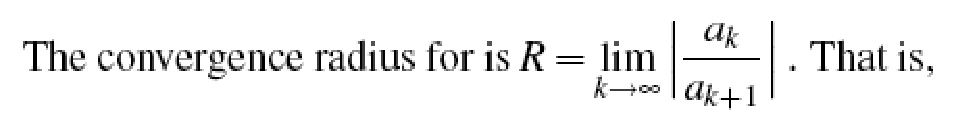
\includegraphics[width=0.55\textwidth]{latex}}}}
\subfigure[由~word软件生成的~.doc~格式行内公式]{\label{word}\fbox{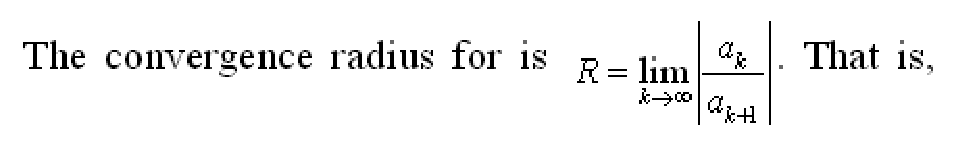
\includegraphics[width=0.55\textwidth]{word}}}
\subfigure[由~word软件生成的~.pdf~格式行内公式]{\label{pdf}\fbox{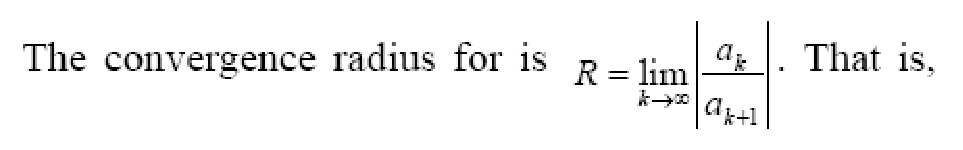
\includegraphics[width=0.55\textwidth]{pdf}}}
\caption{由~\LaTeX~和~word~生成的~3~种行内公式屏显效果}\label{hangju}
\vspace{-1em}
\end{figure}
这三幅图分别为~\LaTeX~和~word~生成的行内公式屏显效果,从图中可看出,在~\LaTeX~文本含有公式的行内,在正文与公式之间对接工整,行距不变;而在~word~文本含有公式的行内,在正文与公式之间对接不齐,行距变大。因此从这一点来说,
\LaTeX~系统在数学公式的排版上具有很大优势。

\LaTeX~提供的行内公式最简单、最有效的方法是采用~\TeX~本来的标记\pozhehao 开始和结束标记都写作~\$,例如本段开始的例子可由下面的输入得到。

\verb|$f(x)=\int_{a}^{b}\frac{\sin{x}}{x}\mathrm{d}x$|

\subsection{行间公式}
位于两行之间的公式称为行间公式,每个公式都是一个单独的段落,例如
\[\int_a^b{f\left(x\right)\mathrm{d}x}=\lim_{\left\|\Delta{x_i}\right\|\to 0}\sum_i{f\left(\xi_i\right)\Delta{x_i}}\]
除人工编号外,\LaTeX~各种类型行间公式的标记见表~\ref{eqtag}。
\begin{table}[htbp]
\caption{各种类型行间公式的标记}\label{eqtag}
\vspace{-0.5em}\centering\zihao{5}
\begin{tabularx}{0.85\textwidth}{cXX}
\toprule
& 无编号 & 自动编号\\\midrule
单行公式 & \verb|\begin{displaymath}...... \end{displaymath}|~或~\verb|\[...\]| & \verb|\begin{equation} ...... \end{equation}|\\
多行公式 & \verb|\begin{eqnarray*} ...... \end{eqnarray*}| & \verb|\begin{eqnarray} ...... \end{eqnarray}|\\
\bottomrule
\end{tabularx}
\end{table}
另外,在自动编号的某行公式行尾添加标签~\verb|\nonumber|,可将该行转换为无编号形式。

行间多行公式需采用~\verb|eqnarray|~或~\verb|eqnarray*|~环境,它默认是一个列格式为~\verb|rcl|~的~3~列矩阵,并且中间列的字号要小一些,因此通常只将需要对齐的运算符号(通常为等号“=”)置于中间列。

\subsection{可自动调整大小的定界符}
若在左右两个定界符之前分别添加命令~\verb|\left|~和~\verb|\right|,则定界符可根据所包围公式大小自动调整其尺寸,这可从式(\ref{nodelimiter})和式(\ref{delimiter})中看出。
\begin{equation}\label{nodelimiter}
(\sum_{k=\frac12}^{N^2})
\end{equation}
\begin{equation}\label{delimiter}
\left(\sum_{k=\frac12}^{N^2}\right)
\end{equation}
式(\ref{nodelimiter})和式(\ref{delimiter})是在~\LaTeX~中分别输入如下代码得到的。
\begin{verbatim}
(\sum_{k=\frac12}^{N^2})
\left(\sum_{k=\frac12}^{N^2}\right)
\end{verbatim}
\verb|\left|~和~\verb|\right|~总是成对出现的,若只需在公式一侧有可自动调整大小的定界符,则只要用“.”代替另一侧那个无需打印出来的定界符即可。

若想获得关于此部分内容的更多信息,可参见~Math mode~文档的第~8~章“Brackets, braces and parentheses”。

\subsection{数学重音符号}
数学重音符号通常用来区分同一字母表示的不同变量,输入方法如下(需要调用~\verb|amsmath|~宏包):

\vspace{0.5em}\noindent\zihao{5}\begin{tabularx}{\textwidth}{Xc|Xc|Xc}
 \verb|\acute| & $\acute{a}$ & \verb|\mathring| & $\mathring{a}$ & \verb|\underbrace| & $\underbrace{a}$ \\
 \verb|\bar| & $\bar{a}$ & \verb|\overbrace| & $\overbrace{a}$ & \verb|\underleftarrow| & $\underleftarrow{a}$ \\
 \verb|\breve| & $\breve{a}$ & \verb|\overleftarrow| & $\overleftarrow{a}$ & \verb|\underleftrightarrow| & $\underleftrightarrow{a}$ \\
 \verb|\check| & $\check{a}$ & \verb|\overleftrightarrow| & $\overleftrightarrow{a}$ & \verb|\underline| & $\underline{a}$ \\
 \verb|\dddot| & $\dddot{a}$ & \verb|\overline| & $\overline{a}$ & \verb|\underrightarrow| & $\underrightarrow{a}$ \\
 \verb|\ddot| & $\ddot{a}$ & \verb|\overrightarrow| & $\overrightarrow{a}$ & \verb|\vec| & $\vec{a}$ \\
 \verb|\dot| & $\dot{a}$ & \verb|\tilde| & $\tilde{a}$ & \verb|\widehat| & $\widehat{a}$ \\
 \verb|\grave| & $\grave{a}$ & \verb|\underbar| & $\underbar{a}$ & \verb|\widetilde| & $\widetilde{a}$ \\
 \verb|\hat| & $\hat{a}$ 
\end{tabularx}\vspace{0.5em}
\zihao{-4} 当需要在字母~$i$~和~$j$~的上方添加重音符号时,为了去掉这两个字母顶上的小点,这两个字母应该分别改用~\verb|\imath|~和~\verb|\jmath|。

如果遇到某些符号不知道该采用什么命令能输出它时,则可通过

http://detexify.kirelabs.org/classify.html~\pozhehao Detexify$^2$~网站来获取符号命令。若用鼠标左键在此网页的方框区域内画出你所要找的符号形状,则会在网页右方列出和你所画符号形状相近的~5~个符号及其相对应的~\LaTeX~输入命令。若所列出的符号中不包括你所要找的符号,还可通过点击“Select from the complete list!”的链接以得分从低到高的顺序列出所有符号及其相对应的~\LaTeX~输入命令。

最后,笔者建议大家还是要以~Math mode~这篇~pdf~文档作为主要参考。若要获得最为标准、美观的数学公式排版形式,可以查查文档中是否有和你所要的排版形式相同或相近的代码段,通过修改代码段以获得你所要的数学公式排版形式。
%% !Mode:: "TeX:UTF-8" 

\section{模板的其它说明}

\subsection{单层罗列环境}
哈工大学位论文一般可采用两种罗列环境:一种是并列条目有同样标签的~\verb|itemize|~罗列环境,另一种是具有自动排序编号符号的~\verb|enumerate|~罗列环境。这两种罗列环境的样式参数可参考图~\ref{list}。
\begin{figure}[htbp]
\centering
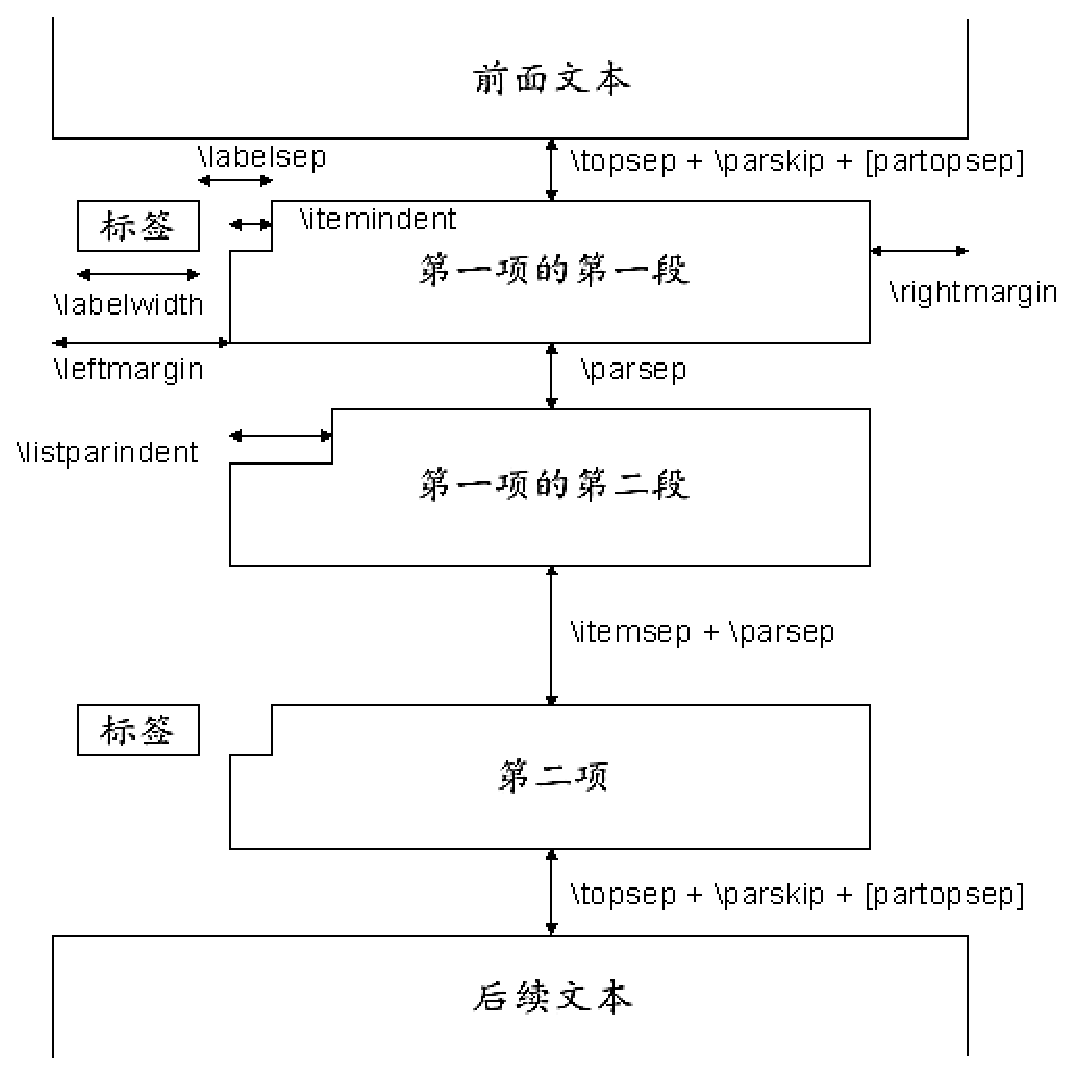
\includegraphics[width = 0.6\textwidth]{list}
\caption{罗列环境参数示意图}\label{list}\vspace{-1em}
\end{figure}
通过调用~enumitem~宏包可以很方便地控制罗列环境的布局,其~format.tex~文件中的~\verb|\setitemize|~和~\verb|\setenumerate|~命令分别用来设置~\verb|itemize|~和~\verb|enumerate|~环境的样式参数。采用~\verb|itemize|~单层罗列环境的排版形式如下:
\begin{itemize}
\item 第一个条目文本内容
\item 第二个条目文本内容
\item 第三个条目文本内容
\end{itemize}
其代码如下
\begin{verbatim}
\begin{itemize}
  \item 第一个条目文本内容
  \item 第二个条目文本内容
  ...
  \item 第三个条目文本内容
\end{itemize}
\end{verbatim}
采用~\verb|enumerate|~单层罗列环境的排版形式如下:
\begin{enumerate}
\item 第一个条目文本内容
\item 第二个条目文本内容
\item 第三个条目文本内容
\end{enumerate}
其代码如下
\begin{verbatim}
\begin{enumerate}
  \item 第一个条目文本内容
  \item 第二个条目文本内容
  ...
  \item 第三个条目文本内容
\end{enumerate}
\end{verbatim}

\subsection{定理定义}

若需要书写定理定义等内容,而且带有顺序编号,需要采用如下环境。除了~\verb|proof|~环境之外,其余~9~个环境都可以有一个可选参数作为附加标题。

\begin{center}\vspace{0.5em}\noindent\zihao{5}\begin{tabularx}{0.7\textwidth}{lX|lX}
定理 & \verb|theorem|~环境 & 定义 & \verb|definition|~环境 \\
例 & \verb|example|~环境 & 算法 & \verb|algo|~环境 \\
公理 & \verb|axiom|~环境 & 命题 & \verb|proposition|~环境 \\
引理 & \verb|lemma|~环境 & 推论 & \verb|corollary|~环境 \\
注解 & \verb|remark|~环境 & 证明 & \verb|proof|~环境 \\
\end{tabularx}\end{center}


\bibliographystyle{GBT7714-2005NLang-HIT}
\addtolength{\bibsep}{-0.8em}
\nocite{*}
\bibliography{reference}

\end{document} 